%%%%%%%%%%%%%%%%%%%%%%%%%%%%%%%%%%%%%%%%%
% Masters/Doctoral Thesis
% LaTeX Template
% Version 2.3 (25/3/16)
%
% This template has been downloaded from:
% http://www.LaTeXTemplates.com
%
% Version 2.x major modifications by:
% Vel (vel@latextemplates.com)
%
% This template is based on a template by:
% Steve Gunn (http://users.ecs.soton.ac.uk/srg/softwaretools/document/templates/)
% Sunil Patel (http://www.sunilpatel.co.uk/thesis-template/)
%
% Template license:
% CC BY-NC-SA 3.0 (http://creativecommons.org/licenses/by-nc-sa/3.0/)
%
%%%%%%%%%%%%%%%%%%%%%%%%%%%%%%%%%%%%%%%%%

%----------------------------------------------------------------------------------------
%	PACKAGES AND OTHER DOCUMENT CONFIGURATIONS
%----------------------------------------------------------------------------------------

\documentclass[
11pt, % The default document font size, options: 10pt, 11pt, 12pt
%oneside, % Two side (alternating margins) for binding by default, uncomment to switch to one side
%chapterinoneline,% Have the chapter title next to the number in one single line
english, % ngerman for German
singlespacing, % Single line spacing, alternatives: onehalfspacing or doublespacing
%draft, % Uncomment to enable draft mode (no pictures, no links, overfull hboxes indicated)
%nolistspacing, % If the document is onehalfspacing or doublespacing, uncomment this to set spacing in lists to single
%liststotoc, % Uncomment to add the list of figures/tables/etc to the table of contents
%toctotoc, % Uncomment to add the main table of contents to the table of contents
%parskip, % Uncomment to add space between paragraphs
%nohyperref, % Uncomment to not load the hyperref package
headsepline, % Uncomment to get a line under the header
]{MastersDoctoralThesis} % The class file specifying the document structure

\usepackage[utf8]{inputenc} % Required for inputting international characters
\usepackage[T1]{fontenc} % Output font encoding for international characters

\usepackage{palatino} % Use the Palatino font by default

\usepackage{graphicx}

%\usepackage[cache=false,outputdir=.texpadtmp]{minted}
\usepackage{minted}

\usepackage[
backend=bibtex,
%style=authoryear,
natbib=true]{biblatex} % Use the bibtex backend with the authoryear citation style (which resembles APA)

\addbibresource{main.bib} % The filename of the bibliography

\usepackage[autostyle=true]{csquotes} % Required to generate language-dependent quotes in the bibliography

%----------------------------------------------------------------------------------------
%	MARGIN SETTINGS
%----------------------------------------------------------------------------------------

\geometry{
	paper=a4paper, % Change to letterpaper for US letter
	inner=2.5cm, % Inner margin
	outer=3.8cm, % Outer margin
	bindingoffset=2cm, % Binding offset
	top=1.5cm, % Top margin
	bottom=1.5cm, % Bottom margin
	%showframe,% show how the type block is set on the page
}

%----------------------------------------------------------------------------------------
%	THESIS INFORMATION
%----------------------------------------------------------------------------------------

\thesistitle{Ÿauhau Extensions to Support Nested Structures, Conditionals and Functions} % Your thesis title, this is used in the title and abstract, print it elsewhere with \ttitle
\supervisor{Sebastian \textsc{Ertel}} % Your supervisor's name, this is used in the title page, print it elsewhere with \supname
\examiner{} % Your examiner's name, this is not currently used anywhere in the template, print it elsewhere with \examname
\degree{Bachelor of Science} % Your degree name, this is used in the title page and abstract, print it elsewhere with \degreename
\author{Justus \textsc{Adam}} % Your name, this is used in the title page and abstract, print it elsewhere with \authorname
\addresses{} % Your address, this is not currently used anywhere in the template, print it elsewhere with \addressname

\subject{Compiler construction} % Your subject area, this is not currently used anywhere in the template, print it elsewhere with \subjectname
\keywords{} % Keywords for your thesis, this is not currently used anywhere in the template, print it elsewhere with \keywordnames
\university{\href{http://tu-dresden.de}{Technische Universität Dresden}} % Your university's name and URL, this is used in the title page and abstract, print it elsewhere with \univname
\department{\href{http://department.university.com}{Chair for Compiler Construction}} % Your department's name and URL, this is used in the title page and abstract, print it elsewhere with \deptname
\group{\href{http://researchgroup.university.com}{Data Flow Optimization Research Group}} % Your research group's name and URL, this is used in the title page, print it elsewhere with \groupname
\faculty{\href{http://inf.tu-dresden.de}{Faculty for Computer Science}} % Your faculty's name and URL, this is used in the title page and abstract, print it elsewhere with \facname

\hypersetup{pdftitle=\ttitle} % Set the PDF's title to your title
\hypersetup{pdfauthor=\authorname} % Set the PDF's author to your name
\hypersetup{pdfkeywords=\keywordnames} % Set the PDF's keywords to your keywords


\newcommand{\fetch}{\texttt{fetch}}
\newcommand{\yauhauPaperTitle}{There is no Applicative: Concise Code and Efficient I/O from Dataflow}
\newcommand{\yauhau}{Ÿauhau}

\begin{document}

\frontmatter % Use roman page numbering style (i, ii, iii, iv...) for the pre-content pages

\pagestyle{plain} % Default to the plain heading style until the thesis style is called for the body content

%----------------------------------------------------------------------------------------
%	TITLE PAGE
%----------------------------------------------------------------------------------------

\begin{titlepage}
\begin{center}

{\scshape\LARGE \univname\par}\vspace{1.5cm} % University name
\textsc{\Large Bachelor Thesis}\\[0.5cm] % Thesis type

\HRule \\[0.4cm] % Horizontal line
{\huge \bfseries \ttitle\par}\vspace{0.4cm} % Thesis title
\HRule \\[1.5cm] % Horizontal line

\begin{minipage}[t]{0.4\textwidth}
\begin{flushleft} \large
\emph{Author:}\\
\href{http://justus.science}{\authorname} % Author name - remove the \href bracket to remove the link
\end{flushleft}
\end{minipage}
\begin{minipage}[t]{0.4\textwidth}
\begin{flushright} \large
\emph{Supervisor:} \\
\href{http://www.jamessmith.com}{\supname} % Supervisor name - remove the \href bracket to remove the link
\end{flushright}
\end{minipage}\\[3cm]

\large \textit{A thesis submitted in fulfillment of the requirements\\ for the degree of \degreename}\\[0.3cm] % University requirement text
\textit{in the}\\[0.4cm]
\groupname\\\deptname\\[2cm] % Research group name and department name

{\large \today}\\[4cm] % Date
%\includegraphics{Logo} % University/department logo - uncomment to place it

\vfill
\end{center}
\end{titlepage}

%----------------------------------------------------------------------------------------
%	DECLARATION PAGE
%----------------------------------------------------------------------------------------

\begin{declaration}
\addchaptertocentry{\authorshipname}

\noindent I, \authorname, declare that this thesis titled, \enquote{\ttitle} and the work presented in it are my own. I confirm that:

\begin{itemize}
\item This work was done wholly or mainly while in candidature for a research degree at this University.
\item Where any part of this thesis has previously been submitted for a degree or any other qualification at this University or any other institution, this has been clearly stated.
\item Where I have consulted the published work of others, this is always clearly attributed.
\item Where I have quoted from the work of others, the source is always given. With the exception of such quotations, this thesis is entirely my own work.
\item I have acknowledged all main sources of help.
\item Where the thesis is based on work done by myself jointly with others, I have made clear exactly what was done by others and what I have contributed myself.\\
\end{itemize}

\noindent Signed:\\
\rule[0.5em]{25em}{0.5pt} % This prints a line for the signature

\noindent Date:\\
\rule[0.5em]{25em}{0.5pt} % This prints a line to write the date
\end{declaration}

\cleardoublepage

%----------------------------------------------------------------------------------------
%	QUOTATION PAGE
%----------------------------------------------------------------------------------------

% \vspace*{0.2\textheight}
%
% \noindent\enquote{\itshape Thanks to my solid academic training, today I can write hundreds of words on virtually any topic without possessing a shred of information, which is how I got a good job in journalism.}\bigbreak
%
% \hfill Dave Barry

%----------------------------------------------------------------------------------------
%	ABSTRACT PAGE
%----------------------------------------------------------------------------------------

\begin{abstract}
\addchaptertocentry{\abstractname} % Add the abstract to the table of contents

Modern large scale, distributed applications require the efficient execution of IO operations such as network or database access.
In this thesis I expand on an idea implemented prior to this in the paper ``\yauhauPaperTitle{}''.
The main focus is generalising its rewrite algorithms to handle alternate flow of control as is present in mapping operations and conditionals.
In addition to that I will provide further evidence for the efficiency achieved in \yauhau{} by conducting experiments on randomly generated program graphs comparing performance with existing solutions.
Lastly I take a look at semantics for effectful actions in the \yauhau{} context, which are writes to your data source.
I will describe issues our dataflow approach introduces into the semantics of writes and how we solve them.

\end{abstract}

%----------------------------------------------------------------------------------------
%	ACKNOWLEDGEMENTS
%----------------------------------------------------------------------------------------

\begin{acknowledgements}
\addchaptertocentry{\acknowledgementname} % Add the acknowledgements to the table of contents

The acknowledgments and the people to thank go here, don't forget to include your project advisor\ldots

\end{acknowledgements}

%----------------------------------------------------------------------------------------
%	LIST OF CONTENTS/FIGURES/TABLES PAGES
%----------------------------------------------------------------------------------------

\tableofcontents % Prints the main table of contents

% \listoffigures % Prints the list of figures
%
% \listoftables % Prints the list of tables

%----------------------------------------------------------------------------------------
%	ABBREVIATIONS
%----------------------------------------------------------------------------------------

\begin{abbreviations}{ll} % Include a list of abbreviations (a table of two columns)

\textbf{IO} & \textbf{I}nput/\textbf{O}utput\\
\textbf{IR} & \textbf{I}ntermediate \textbf{R}epresentation (of a program)\\
\textbf{DLS} & \textbf{D}omain \textbf{S}pecific \textbf{L}anguage\\
\textbf{EDLS} & \textbf{E}mbedded \textbf{D}omain \textbf{S}pecific \textbf{L}anguage\\
\textbf{DAG} & \textbf{D}irected \textbf{A}cyclic \textbf{G}raph\\

\end{abbreviations}

%----------------------------------------------------------------------------------------
%	PHYSICAL CONSTANTS/OTHER DEFINITIONS
%----------------------------------------------------------------------------------------

% \begin{constants}{lr@{${}={}$}l} % The list of physical constants is a three column table
%
% % The \SI{}{} command is provided by the siunitx package, see its documentation for instructions on how to use it
%
% 	Speed of Light & $c_{0}$ & \SI{2.99792458e8}{\meter\per\second} (exact)\\
% %Constant Name & $Symbol$ & $Constant Value$ with units\\
%
% \end{constants}

%----------------------------------------------------------------------------------------
%	SYMBOLS
%----------------------------------------------------------------------------------------

% \begin{symbols}{lll} % Include a list of Symbols (a three column table)
%
% $a$ & distance & \si{\meter} \\
% $P$ & power & \si{\watt} (\si{\joule\per\second}) \\
% %Symbol & Name & Unit \\
%
% \addlinespace % Gap to separate the Roman symbols from the Greek
%
% $\omega$ & angular frequency & \si{\radian} \\
%
% \end{symbols}

%----------------------------------------------------------------------------------------
%	DEDICATION
%----------------------------------------------------------------------------------------

\dedicatory{For/Dedicated to/To my\ldots}

%----------------------------------------------------------------------------------------
%	THESIS CONTENT - CHAPTERS
%----------------------------------------------------------------------------------------

\mainmatter % Begin numeric (1,2,3...) page numbering

\pagestyle{thesis} % Return the page headers back to the "thesis" style

% Include the chapters of the thesis as separate files from the Chapters folder
% Uncomment the lines as you write the chapters


%!TEX root = ../thesis.tex
\chapter{Introduction}

\label{ch:Intro}


% TODO the intro is a bit twisted: normally an intro goes by this structure: problem, missing solutions, contributions, outline (I like it when the last two are co-mingled.)

This thesis concerns itself with the extension and improvement of \yauhau{}, an IO optimisation compiler plugin for the Ohua framework.
\yauhau{} was first introduced in the paper ``Ÿauhau: Concise Code and Efficient I/O Straight from Dataflow.''~\cite{ErtelGoensAdamEtAl2016}.
In the paper, which was written by Sebastian Ertel, Andrés Goens, Jeronimo Castrillon and myself, we explained how \yauhau{} rewrites a program to achieve efficient IO whilst allowing the programmer to write very concise and straight forward code.
We also alluded to some of the issues that arise from control flow when performing the \yauhau{} transformation and we briefly outlined the solutions that we developed.

In this thesis I want to explain in much more detail the concrete ways in which I handle control flow in \yauhau{} and explain implementation considerations and decisions made during and after writing of the paper but which we unfortunately did not have space for in the paper itself.
Chapter~\ref{ch:smap-transformation} concerns itself with \texttt{smap} and Chapter~\ref{ch:if-transformation} explains in more detail the handling of \texttt{if}.
I also want to introduce the reader to a new generalised concept, called context (Chapter~\ref{ch:Context}), which has now been added to Ohua and allows the correct handling of nested control flow structures.
After that in Chapter\ref{ch:trans-implementation} I will briefly describe some general implementation decisions for \yauhau{} and optimisations which were added.

Following the contexts I will introduce another recent addition to \yauhau{} which we hinted at briefly in the paper, side effects and how to handle them semantically (Chapter\ref{ch:side-effects}).
This chapter introduces the concept of controlled side effects in a functional and parallel system such as Ohua by means of the \yauhau{} plugin and how we intend to preserve semantics with regards to caching as well as read-write conflicts, whilst enabling easy and straight forward modularity.

At the beginning however I will introduce the reader to the underlying Ohua framework (Chapter~\ref{ch:Ohua}) and the basics of the \yauhau{}~\ref{ch:Yauhau} plugin, the latter of which includes a description of the basic IO batching transformation.

Contributions of this thesis are:
\begin{itemize}
    \item A more detailed description, including implementation considerations and decisions, of the \textbf{if and smap transformations}.
    \item The generalisation of non structurally emergent dataflow graph properties into a concept called \textbf{Context}, its detection and use to handle nested control flow in \yauhau{}.
    \item An optional graph transformation in \yauhau{} used to \textbf{preserve write semantics} in programs using the \yauhau{} batching.
    \item An evaluation of the effect of precomputed conditional branches on latency.
    \item New \textbf{experiments} showing the performance of the \yauhau{} plugin in comparison to the existing technologies Haxl and Muse in \textbf{programs with conditionals and mapping}.
    \item \textbf{Extensions to the random code generator}~\cite{Goens-rand-code-graph} used in the \yauhau{} paper to generate test programs.
    These extenstions enable \textbf{support for mapping operations} as well as different \textbf{generation methods for conditionals} in the code generator.
\end{itemize}

%
% This thesis intends to improve on the current implementation of this plugin, provide explanation as to why adjustments to the implemetation are necessary in the first place, document adjustments made to the Ohua core which enable the plugin to function and finally expand on the experimental evaluation started in the paper, providing comparative data for performance of our plugin against frameworks with similar functionality.
%
% \section{Fundamental Technologies}
%
% This section shall serve as a reference for technologies which this thesis and its implementation is based upon.
% After this section I presume the reader to be familiar with these technologies and concepts and shall not provide further explanation.
%
% \subsection{Clojure}
%
% Clojure is a functional, dynamically typed language targeting the JVM  which we use to express the higher level algorithms in Ohua.
% Bejond that I use Clojure to implement most of the compiler internal algorithms, including those described in this thesis.
% There will occasionally be code examples to illustrate certain algorithms I am describing, those will usually be written in the Clojure language.
%
% \subsection{Ohua}
%
% Ohua is an automated parallelization framework which combines low level efficiency as provided by the JVM with high level expressions as found in the clojure programming language.
% In Ohua algorithms are implemented in the expressive clojure language and in terms of so called stateful functions, performant and state heavy java code pieces.
% Algorithms implemented in this way will can be automatically disassembled into a data flow graph and parallelized by the Ohua runtime and scheduler.

%% Chapter Template

\chapter{Selected data flow fundamentals} % Main chapter title

\label{ChapterDataFlow} % Change X to a consecutive number; for referencing this chapter elsewhere, use \ref{ChapterX}

%----------------------------------------------------------------------------------------
%	SECTION 1
%----------------------------------------------------------------------------------------

\section{Graph representation}

Bindings:

read

write

\subsection{Implementation}

\subsection{Interpretation}

The aforementioned graph implementation can be interpreted as a directed, acyclic graph.
The direction is given by the flow of data, from output to input.
The graphhas to be acyclic.
This is a restriction currently imposed by the underlying Ohua framework but it is also embraced by the algorithms in this thesis because it allows simpler implementations.
Functions are nodes.
I hereby mean a function as a concrete invocation including input and output bindings.
This is in contrast to \textit{function names} which are simply labels to the node describing its functionality.
Bindings are edges.
Each named binding can represent or indicate multiple or no edges.
Bindings are \textit{write once}, hence any binding may only occur once as a return value but may be used an arbitrary number of times as input value.
As a result all edges represented by a particular binding originate from the same node.
Furthermore the graph must be complete, as in any binding read must have previously been written.
For each time a binding is read it represents an edge from its source node to the reading node.
Thus a binding which is never read creates no edges.

%% Chapter Template

\chapter{Context handling} % Main chapter title

\label{ChapterContext} % Change X to a consecutive number; for referencing this chapter elsewhere, use \ref{ChapterX}

%----------------------------------------------------------------------------------------
%	SECTION 1
%----------------------------------------------------------------------------------------

\section{What is Context?}

A context, as far as Ohua is concerned, is a programming construct which changes the behavior of subsequent sections of code.
As an example the most basic context is the root context of an ohua \textt{algo} which changes the behavior of the functions within in so far as that they are executed once for each time the algo is executed.
Another example is the \texttt{smap} context which casues functions within to be executet multiple times.
Both of these contexts are control flow contexts which means they alter whether and how often functions are executed.
Most contexts in ohua are represented as a pair of encapsulating operators which mark the beginning and end of the context respectively and the context itself influences the operators in between.
The beginning marker sets up the altered behaviour and the end marker restores the original behavior.

In case of the \texttt{algo} context the \texttt{algo-in} as start operator starts the execution and the \texttt{algo-out} operator as end operator collects the result.
For \texttt{smap} the \texttt{smap} operator starts by executing the algorithm within once for each element in the structure being mapped and the \texttt{collect} operator restores the old behavior by waiting for as many elements as were in the mapped structure before returning them collectively to the next part of the program.

\subsection{Arising problems}


Control flow altering context such as smap or if pose a problem for yauhau.
The idea behind our batching transformation is to find sets of pairiwise independant fetches and replacing them with a single, accumulated (batched) fetch.
The accumulator would execute all fetches at once and return the results back into the appropriate place in the graph.
However it is a simple operator and has to wait for all inputs before executing.
This would pose an issue, were one of its inputs coming from the branch of a conditional, such as if.
If the branch in question was not selected at runtime the input to the accumulator would be missing, preventing it from executing any of the fetches.
Similarly with the map operation smap.
Were one of the inputs to the accumulator originating from inside an smap the input could get several values instead of just one, a situation which the naive accumulator is unable to cope with.
As a result we need to ensure all inputs to an accumulator are present at the same time and in the same quantity.
In turn this means each of the pairwise parallel fetches has to be called the same number of times.
The simplest way to do this is to remove all control flow context around a fetch operation, leaving it in the root context.
Here we are guaranteed that any fetch will only ever be executed once.

I should mention that there is an alternative strategy for handling this but it would require runtime scheduling.
Scheduling offers more flexibility but at the same time also poses a substantially larger runtime overhead.
Because of this we opted for a compile time rewrite approach.

Haxl and muse both use runtime techniques to tackle this problem.
In the case of Haxl it leverages the Haskell runtime (scheduler) whereas muse relies on a runtime AST and traversals on this AST.

\subsubsection{}

%-----------------------------------
%	SUBSECTION 1
%-----------------------------------
\subsection{Definition}

We define

%-----------------------------------
%	SUBSECTION 2
%-----------------------------------

%\chapter{Handling Context in \yauhau}

\label{ChapterRewrites}

\section{Anterior considerations} % TODO Find a better title

Changes made to the program graph in \yauhau{} naturally succeed the context recognition step.
Changes made may include removing nodes from the program graph, or inserting new nodes.
Particularly dangerous is the insertion of new nodes, since at this stage we are not dealing with a simple list of funtions\footnote{As described in the section about the Ohua IR.} but a labeled graph with information about contexts to functions.
Subsequent compiler steps may wish to access the context information also hence we must preserve it, though at present none such compiler steps are implemented or planned.
Furthermore when inserting nodes we must assign correct context information to the newly inserted nodes.

A simple but inefficient way would be to unlabel and relabel the graph every time we make a significant change.
Since the labeling is not particularly cheap this seams inadvisable.
We therefore presume the rewrite implementer to provide appropriate context labels for inserted nodes himself.

\subsection{Providing appropriate context labels}

Assuring labels for nodes inserted after labeling the graph are correct is a hard problem. % TODO how hard?

In the concrete use case of \yauhau{} however we can leverage additional information about the kind of nodes we insert and derive universal properties for these functions which simplify the labeling process.

%!TEX root = ../thesis.tex
\chapter{Ohua}

\label{ch:Ohua}

Ohua\cite{Ertel:2015:OID:2807426.2807431}\cite{Ohua:library:link} is parallelisation framework implemented in Java\cite{JavaLanguage} and Clojure\cite{ClojureLanguage}.

At compile time Ohua transforms the program into a dataflow graph.
This graph is a representation of individual chunks of code of the program and the data dependencies between them.
Since Ohua currently does not support recursion this graph is a DAG.
Nodes are atomic pieces of code which are called stateful functions.
Edges represent data dependencies.
Edge direction indicates result and argument.
The result of the source node is argument to the target node.
The result value of one stateful function may be used by multiple other stateful functions and each stateful function can have multiple inputs or none at all.
An example of how this transformation looks can be seen in Figure~\ref{fig:ohua-code-example}.
All of the called functions here, such as \texttt{vector}, \texttt{add} etc. have to be implemented as stateful functions, see Figure~\ref{fig:ohua-sfn-example}.

\begin{figure}[h]
\begin{minted}{Clojure}
(def main
  (ohua
    (let [a (increment 1)
          b (add 2 a)
          c (some-action)]
      (vector a b c))))
\end{minted}
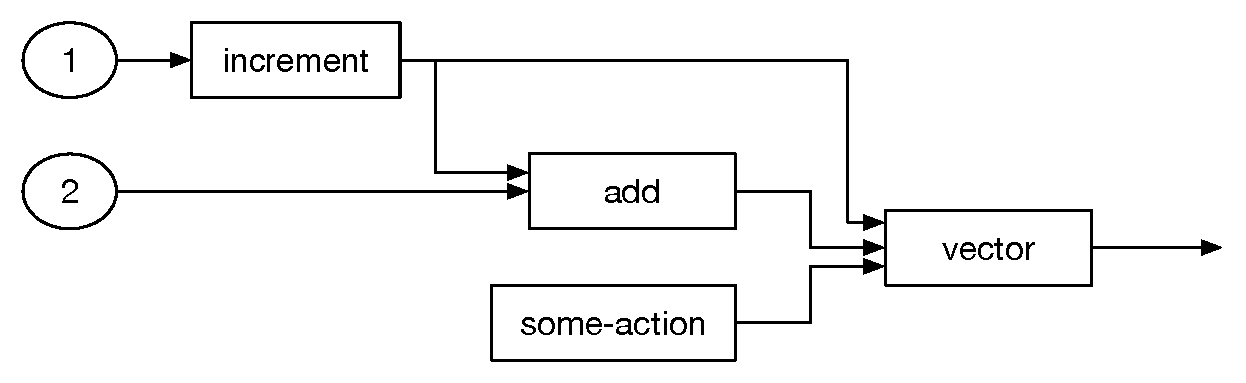
\includegraphics[width=\linewidth]{../Figures/ohua-code-example}
\caption{An example for code transformation in Ohua}
\label{fig:ohua-code-example}
\end{figure}

\begin{figure}[h]
\begin{minted}{Java}
public class Add {
  @defsfn // <- the annotation to make a stateful function
  public Int add(Int i1, Int i2) {
    return i1 + i2;
  }
}
\end{minted}
\caption{Example implementation for \texttt{add}}
\label{fig:ohua-sfn-example}
\end{figure}

This dataflow graph can then be executed by a dataflow execution runtime which dynamically schedules the nodes of the graph.
The runtime knows about the data dependencies between the nodes of the graph and therefore can schedule independent nodes in parallel.
Data independent nodes can be executed in parallel.
Also subsequent calls to the same node with unrelated data, as a result of a mapping operation for instance, can be executed in parallel.
This property allows us to do deterministic state modifications on an object of the class the stateful function is attached to.
As a result we obtain pipeline parallelism.


\begin{figure}
  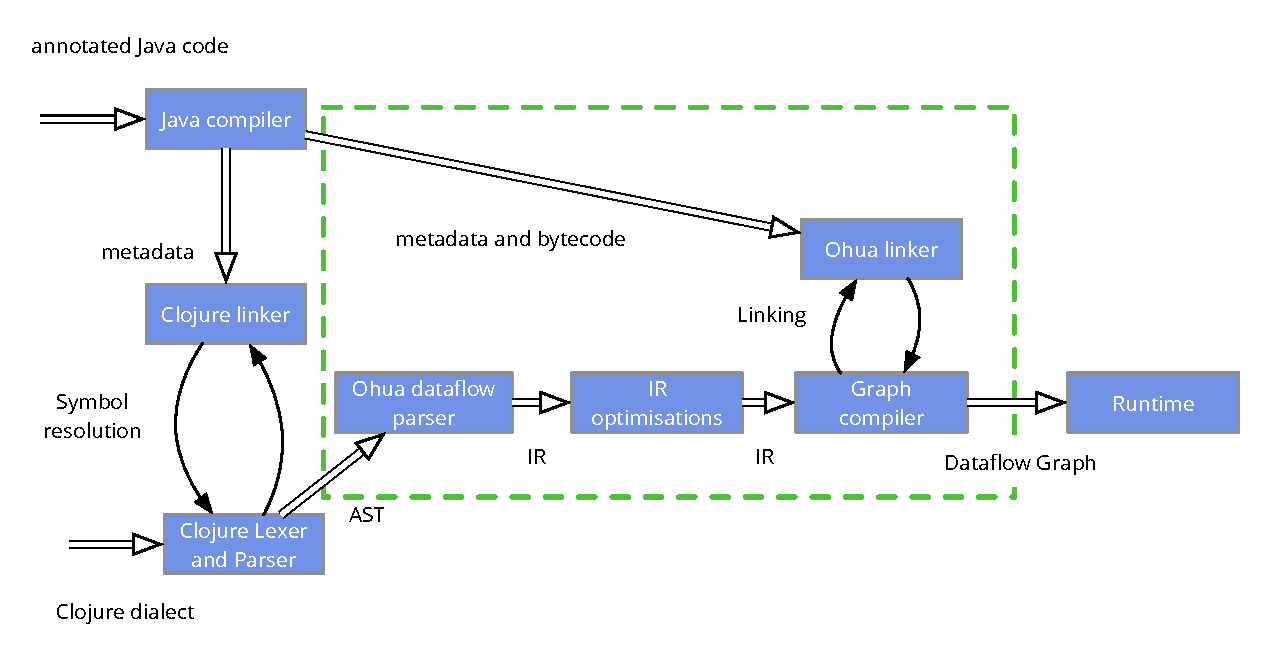
\includegraphics[width=\linewidth]{../Figures/ohua-compiler-flow}
  \caption{Compiler flow of Ohua}
  \label{fig:ohua-compiler-flow}
\end{figure}


\section{Stateful Functions}


Stateful functions are the nodes of the Ohua dataflow graph.
They represent atomic pieces of code which the Ohua runtime schedules.
Stateful functions can be implemented in Java by annotating a method with \texttt{@defsfn}, or in Clojure by using the \texttt{defsfn} macro.
Each stateful function has an associated class, which holds the internal, opaque state of the node.
Whenever a stateful function is referenced in code in the \texttt{ohua} or \texttt{algo} macro the runtime creates a new instance of the class in which the stateful function is implemented.
As a result invocations of the same call site of a stateful function share an opaque state.
But different call sites do not share state implicitly.
To share state across call sites the state has to be explicitly passed to the function as an argument.
This ensures that state sharing is transparent to the runtime without requiring in depth knowledge about the structure of the state itself.

When executing the dataflow graph the runtime dynamically executes nodes.
As a result the precise order in which the graph is executed is indeterministic.
However the runtime ensures that for each node the order of its subsequent invocations is preserved which ensures correct semantics not only in the high level algorithm but also with regards to the internal, opaque state of the stateful function itself.

\section{Algorithms}

Algorithms express high level, parallelisable computations in Ohua.
These algorithms are written in Ohua's Clojure EDSL using the \texttt{algo} macro.
Algorithms use and combine stateful functions to express complex computations.
Algorithms are generally assumed to be pure in so far as there are no data dependencies between any two functions which are not directly visible via function arguments and return values.
No two functions should share data in any way other then by explicitly passing them from one to the other via arguments and result.
Furthermore there should not be any dependency on invocation ordering which is not expressed directly through data dependencies.
The snippet of code in Figure~\ref{fig:indeterministic-code} for example: If this were normal Clojure code, the read would be executed before the write due to the sequential, deterministic semantics of a Clojure \texttt{let} binding.
In Ohua however, since there are no data dependencies between \texttt{read} and \texttt{write}, the execution order of those two stateful functions is nondeterministic and they could even be executed simultaneously.
The graph in Figure~\ref{fig:indeterministic-code} shows very nicely how at this stage there is no visible order for those two actions in the compiled graph.
When the algorithm is executed using the \texttt{ohua} or \texttt{<-ohua} macro the algorithms Clojure code is compiled into a dataflow graph and executed by the Ohua runtime.

\begin{figure}
\begingroup
\definecolor{green(html/cssgreen)}{rgb}{0.0, 0.5, 0.0}
\catcode`\@=\active
\def@#1@{\textcolor{green(html/cssgreen)}{#1}}
\begin{minted}[escapeinside=||]{Clojure}
(|@defalgo@| my-algo []
  (let [a (read-database)
        b (write-database)]
    (compute a b)))
\end{minted}
\endgroup
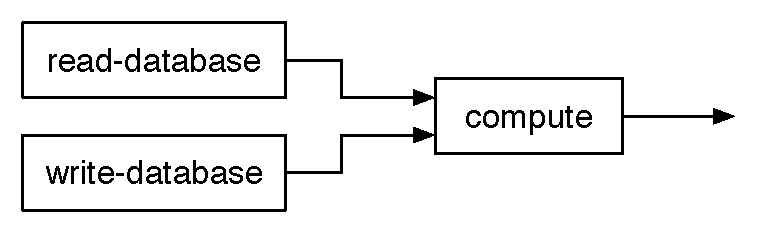
\includegraphics[width=\linewidth]{../Figures/indeterministic-code-example}
\caption{An example of indeterministic code}
\label{fig:indeterministic-code}
\end{figure}

\section{Dataflow IR}

Ohua was already using a data flow graph for its runtime execution model, but in order to implement Yauhau we also needed a (much simpler) compile time data flow graph representation.
A simplified dataflow representation also lends itself nicely for performing high level optimisations on the graph itself as well as perform analysis such as type checking\footnote{This may be subject of future work}.
As a result the dataflow IR on which \yauhau{} operates is now directly part of Ohua and its compilation pipeline.

Like the final dataflow graph the IR encodes the dataflow relationships inside of the program.
The description of the graph contains two elements:

\begin{enumerate}
    \item \textbf{Bindings} are named data elements or alternatively can be interpreted as a data path.
    Each binding has to be unique and constant, which means it can only be assigned once, in which case we also speak of the \textit{creation} of the binding or of \textit{writing} the binding.
    However the binding may be read any number of times (including 0).
    \item \textbf{Functions} represent call sites of stateful functions.
    A function name references the stateful function which should be called.
    A list of input, or parameter, bindings references the data which is expected as argument to the stateful function and a list of result bindings creates references to the data produced by the stateful function.
    The same stateful function can be referenced by multiple IR functions, since IR functions represent call sites of a stateful function, not the stateful function itself.
    If a binding is present in a parameter list we also speak of the binding being \textit{read}.
    Is the binding present in the result bindings list we also speak of the binding being \textit{written} or \textit{created}\footnote{Due to the uniqueness constraint \textit{writing} and \textit{creating} are the same here.}.
\end{enumerate}

Any IR graph can be easily serialised into a Clojure \texttt{let} form preserving the semantics of the graph.
The serialisation of the dataflow IR into a human readable form makes it easy to reason about semantics of the program, which in turn makes it easier for a programmer to debug the program.
Additionally theoretical validity of a graph can be shown by showing that the corresponding Clojure program is valid.

\subsection{Implementation}

The actual implementation of the graph is simply a list of functions, see Figure~\ref{fig:concrete-ir-snippet}.
Each function is a Clojure record with fields for a unique id, the name of the function, a vector of input bindings and a binding or a vector of bindings as result values.
By moving result lists to the left and a putting a Clojure function call to the right this graph can be represented as a Clojure \texttt{let} form, see Figure~\ref{fig:ir-as-clojure}.

\begin{figure}[h]
\begin{minted}{Clojure}
(defrecord IRFunc [id name args return])

(def graph
	[(->IRFunc 1 "f" ['a 'b] 'c)
	 (->IRFunc 2 "g" ['c] ['d 'e])])

\end{minted}
\caption{Concrete IR snippet}
\label{fig:concrete-ir-snippet}
\begin{minted}{Clojure}
(let [c (f a b)
      [d e] (g c)]
  [d e])
\end{minted}
\caption{IR representation as Clojure program}
\label{fig:ir-as-clojure}
\end{figure}

% \subsection{Interpretation}
%
% This IR encodes a DAG.
% The direction is given by the flow of data, from output to input.
% The graphs have to be acyclic.
% This is a restriction currently imposed by the underlying Ohua framework but it is also embraced by the algorithms in this thesis because it allows simpler implementations.
% In the future this restriction may be lifted, at least internally, to allow more optimisations and flexibility.
%
% Functions are nodes.
% I hereby mean a function as a concrete call site including input and output bindings.
% This is in contrast to \textit{function names} which are simply labels to the node describing its functionality.
%
% Bindings are edges.
% Each named binding represents multiple edges, including none.
% Bindings are \textit{write once}, hence any binding may only occur once as a result value but may be used an arbitrary number of times as input value.
% As a result all edges represented by a particular binding originate from the same node.
% Furthermore the graph must be complete, as in any binding read must have previously been written.
% For each time a binding is read it represents an edge from its source node to the reading node.
% Thus a binding which is never read creates no edges.
% For conversion into an executable Ohua graph the ordering of functions in the IR is irrelevant, no topological sort is required.

%!TEX root = ../thesis.tex
\chapter{Yauhau}

\label{ch:Yauhau}

\yauhau{} is a plugin for the Ohua compiler.
Following I will briefly outline the basic transformation in \yauhau{} which is necessary to understand the arising problems which I am solving in the Chapters following.

\yauhau{} hooks into the compiler after the Clojure source has been parsed and transformed into the dataflow IR.
It is a pure IR to IR transformation.
In the flow graph in Figure~\ref{fig:ohua-compiler-flow} \yauhau{} would be run as part of the IR optimisation step.
Additionally a map of context information is given to the plugin.
The precise nature of this context information will be explained in section \ref{ch:Context} its information is used in the transformations of Chapter~\ref{ch:if-transformation} and Chapter~\ref{ch:smap-transformation}.
It is irrelevant to the basic \yauhau{} idea and transformation.

Fundamentally \yauhau{} performs a graph transformation on the dataflow graph it has been given in form of the IR.
The goal behind this transformation is to find sets of I/O operations which are data independent from each other.
This is functionally similar to the approach taken by Haxl\cite{Haxl:library:link}, see Chapter~\ref{ch:related-work}.
Haxl leverages the Monad and Applicative abstractions provided by the Haskell language and base library to propagate a list of parallel executable I/O actions through the program path, blocking each path as soon as an I/O action is encountered.
This is a dynamic way of finding parallel I/O actions, i.e. at runtime a data structure (Data.Sequence.Seq) is populated with pending requests.
\yauhau{} takes a different approach and statically finds parallel I/O actions at compile time.

\begin{figure}
    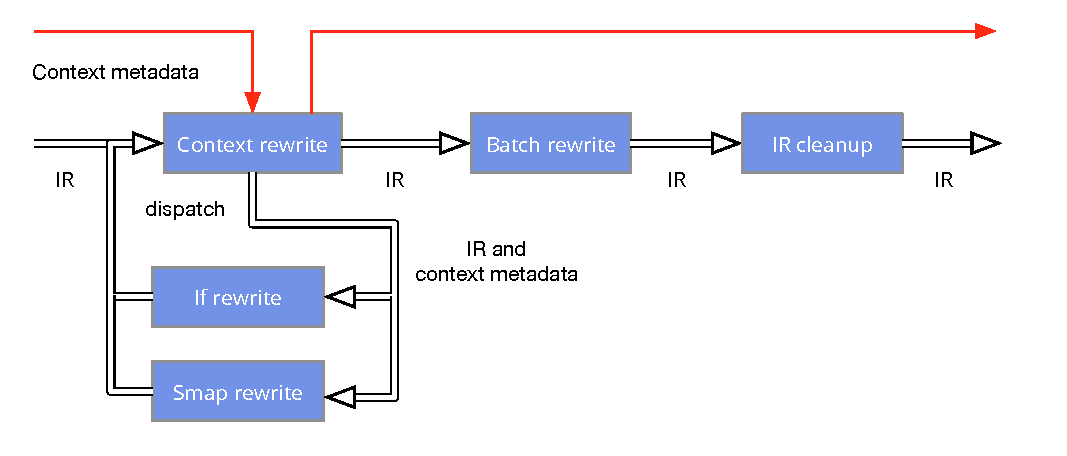
\includegraphics[width=\textwidth]{../Figures/yauhau-rewrite-flow}
    \caption{Rewrite order and flow in \yauhau{}}
    \label{fig:yauhau-rewrite-flow}
\end{figure}

You can see the full \yauhau{} transformation flow in Figure~\ref{fig:yauhau-rewrite-flow}.
We will discuss the individual parts of this flow graph in the upcoming sections.

\section{Runtime execution}

In \yauhau{} an accumulative fetch node, called \texttt{\_\_accum-fetch} statically replaces a set of fetches.
This is equivalent to a \textbf{round} in Haxl.
The accumulator is statically wired into the call sites of the fetches it replaces.
It has one input and one output for each \texttt{fetch} node it replaces.
Once a request for each input is present at runtime the accumulator executes, retrieving all of the requests simultaneously.

The parallel fetches are grouped into sequences of fetches on the same data source.
Each sequence is handed to its respective data source which has to perform the fetch.
In \yauhau{} this process is inherently parallel and each data source performs its request simultaneously.
In Haxl the programmer can choose whether to perform an asynchronous or synchronous request.
When all data sources are finished the results are distributed back through the corresponding outputs of the accumulator.
A visual representation of this can be seen in Figure~\ref{fig:yauhau-transformation}.

A new experimental and optional feature in \yauhau{} is to do dynamic dispatching of the finished requests.
This means once a certain data source returns with the data, computations only depending on that data source, can continue immediately.

\section{Data sources}

Similar to Haxl, compare Section~\ref{subs:datasources}, all data sources a user wants to access in \yauhau{} must be defined externally.

\yauhau{} has a more loose way of working with data sources than Haxl.
I/O actions in \yauhau{} are instances of the \texttt{Request} class.

\begin{figure}[h]
\begin{minted}{Java}
class Request<Payload, Return>{
  Paylod payload;
  IDataSource<Payload, Return> dataSource;
  Request(Payload payload,
          IDataSource<Payload, Return> dataSource)
    { /* implementation omitted */ }
  /* omitted code */
}
\end{minted}
\caption{Implementation of the \texttt{Request} class}
\label{fig:request-class-implementation}
\end{figure}

Each \texttt{Request} has two fields, an arbitrary Payload and a data source, compare Figure~\ref{fig:request-class-implementation} .
Here the data source, similarly to Haxl implements a Java interface \texttt{IDataSource}, see Figure~\ref{fig:idatasource-interface-implementation}, which provides a method for executing batched requests, hence the type \texttt{Iterable<Payload>} for the \texttt{fetch} method on the \texttt{IDataSource} interface (Figure~\ref{fig:idatasource-interface-implementation}   ).

\begin{figure}[h]
\begin{minted}{Java}
interface IDataSource<Payload, Return> {
  Object getIdentifier();
  Iterable<Return> fetch(Iterable<Payload> requests);
}
\end{minted}
\caption{Implementation of the \texttt{IDataSource} interface}
\label{fig:idatasource-interface-implementation}
\end{figure}

At runtime requests are grouped by the data source they are paired with and then handed to the respective source as a single sequence of many requests.

\section{Compile time transformation}

The basic \yauhau{} transformation, as mentioned, operates entirely on a dataflow graph.
The transformation does not concern itself with the kinds of nodes in the graph except for one, the \texttt{fetch} node/function which is a special node provided by the \yauhau{} library.
Beyond that, to simplify the transformation, it operates exclusively on the structure of the graph.
The \fetch{} node itself is implemented as a regular stateful function (See Figure~\ref{fig:fetch-implementation}) and works without the \yauhau{} transformation, although using it without the batching optimisation makes it much less useful.
Since data sources expect sequences of requests the \texttt{fetch} operator builds one and then returns the first element from the sequence of results returned by the data source.
If the source works as expected this result sequence should hold results of performing the requests in the same order as the requests were originally.

\begin{figure}[h]
\begin{minted}{Java}
class FetchOp<P, R> {
  @defsfn
  R fetch(Request<P, R> request) {
    List<P> l = Collections.singletonList(
                  request.getPayload()
                );
    Iterable<R> res = request.getDataSource().fetch(l);
    return res.iterator().next();
  }
}
\end{minted}
\caption{implementation of the \texttt{fetch} stateful function}
\label{fig:fetch-implementation}
\end{figure}

\subsection{Round detection}

The goal of the round detection is to find a minimal set of rounds.
A `round' is a set of \texttt{fetch} nodes with no data dependencies between the nodes.
Rounds must not overlap.
Hence the round detection finds a minimal set of non overlapping sets of data independent \texttt{fetch} nodes.

\subsubsection{Algorithm description}

To find the rounds in a given program I simulate the execution of the program and block code paths when a \texttt{fetch} node is encountered.
The simulation is done by topologically visiting the nodes of the graph while tracking three sets of items.

\begin{description}
	\item[created] The set of created bindings tracks which pieces of data that flow between the nodes of the program have been created prior to a particular point in the program.
	\item[visited] The set of visited nodes tracks which nodes were part of a previous stage.
	\item[round] The current round consists of all pending \fetch{} nodes.
	When a new fetch round is finalised it will consist of these \fetch{} nodes and the current round will be newly initialised empty.
\end{description}

Since bindings are unique in the dataflow IR we can track produced data by simply adding the respective binding to the set of created bindings.
The set of created bindings is initialised with the input parameters of our program.
From this point we traverse the graph in stages.
Each stage consists of the set of graph nodes where all inflowing data has previously been created and which was not in a previous stage.

For the former condition we check, for each input binding, whether the respective binding is contained in the set of \emph{created} bindings.
To ensure the latter condition a separate set of \emph{visited} nodes is maintained and only nodes which are not members of this set are allowed in a new stage.
Once the stage has been computed all functions in the stage are added to the \emph{visited} set.
Then all \fetch{} nodes are filtered from the stage and added to the current \emph{round}.
All remaining nodes are being executed.
Simulating to executing the nodes is done by simply adding all produced bindings (return bindings) of the node to the \emph{created} set.
If there are no remaining nodes to execute in a stage we have reached a point where the remainder of the dataflow graph depends on I/O actions, including the \fetch{} nodes.
Therefore the current round is maximal and we simulate executing all \texttt{fetch} nodes of the current round and dispatch a finalised fetch round.
Afterwards the current \emph{round} set is initialised empty again.
This is done until we get an empty stage, at which point we dispatch the current round again, unless it is empty, and we have reached the end of the round detection.

\begin{figure}
    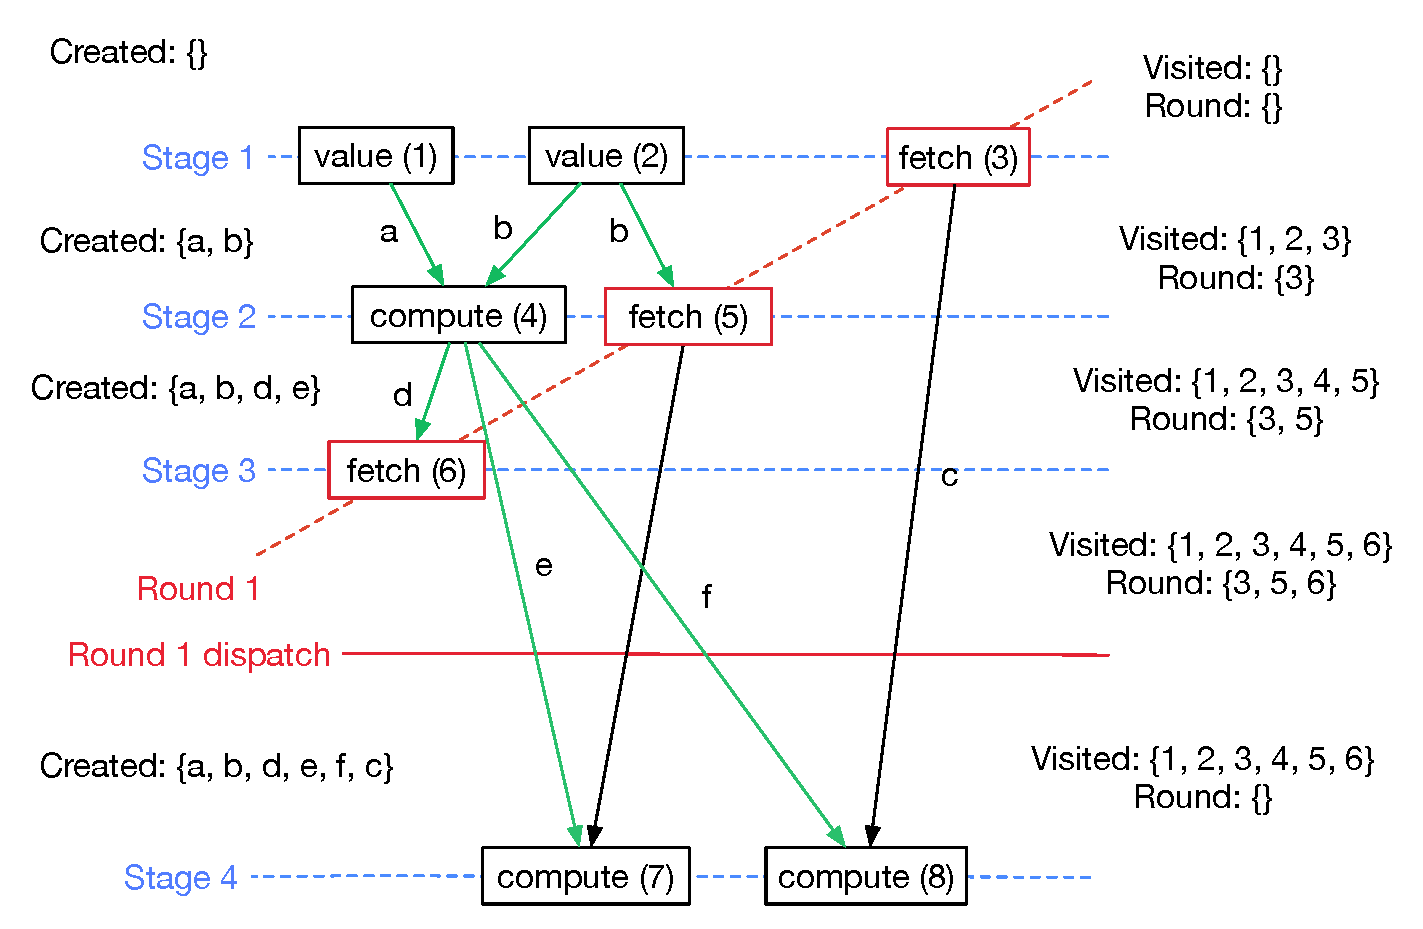
\includegraphics[width=\textwidth]{yauhau-round-detection}
    \caption{Example of the round detection algorithm}
    \label{fig:yauhau-round-detection}
\end{figure}

As an example you can see a typical dataflow IR graph in Figure~\ref{fig:yauhau-round-detection}.
The number after the node name is the unique id for that particular node and used for in the \emph{Visited} and \emph{Round} sets.
Blue dotted lines mark the stages as we traverse the graph.
In each stage only nodes for whom all incoming edges are created, symbolised, for up to the first round, by the green arrows, can be part of the stage.
You can also follow this algorithm along in Figure~\ref{fig:round-detection}.
After each stage the outgoing nodes are added to the created set as seen on the lefthand side.
The red \fetch{} nodes block the propagation through the graph and they are added to the \emph{Round} set on the righthand side.
After stage three we have no more nodes for whom all incoming edges are green, and therefore we dispatch a round of fetches, indicated by the dotted red line.
When the round has been dispatched, indicated by the solid red line, its created bindings are added to the \emph{Created}, visible after the dispatch on the lefthand side.

\begin{figure}
\textbf{Remarks:}
\begin{itemize}
  \item \texttt{set/union} is the set-union ($\cup$), \texttt{set/difference} is the set-difference ($\setminus$) and \texttt{\#\{\}} is an empty set.
  \item \texttt{filter} filters the collection where the predicate is true, \texttt{remove} where the predicate is false.
  \item \texttt{loop} and \texttt{recur} is tail recursion in clojure.
    \texttt{recur} restarts the body of \texttt{loop} with variables bound to the arguments of \texttt{recur}.
  \item \texttt{ir} is the ir graph give to the algorithm
\end{itemize}
\begin{minted}{Clojure}
(loop [visited #{}
       created #{}
       round #{}
       rounds []]
  (let [stage (set/difference
                (get-callable-fns created ir)
                visited)
        new-visited (set/union visited stage)]
    (if (empty? stage)
      ; end algorithm
      (if (empty? round)
        rounds
        (conj rounds round))
      ; continue
      (let [fetches (filter is-fetch? stage)
            non-fetches (remove is-fetch? stage)
            new-round (set/union round fetches)]
        (if (empty? non-fetches)
          ; dispatch round
          (recur new-visited
                 (set/union
                   created
                   (all-return-bindings new-round))
                 ; next round set to empty again
                 #{}
                 ; current round appended to rounds
                 (conj rounds new-round))
         ; continue to next stage
         (recur new-visited
                ; non-fetch bindings are now created
                (set/union
                  created
                  (all-return-bindings non-fetches))
                new-round
                rounds)))))
\end{minted}
\caption{Round detection algorithm in Clojure}
\label{fig:round-detection}
\end{figure}

\subsubsection{Result guarantees}

Adding the \fetch{} nodes to the set of visited nodes guarantees that rounds do not overlap.
Not simulating fetch execution before the round finishes guarantees that no round contains two fetches with data dependencies between them, since the dependent fetch would never have been in a stage before the round was finished since the required binding from the first fetch would not be created before the round finishes.
Finally since we only dispatch a round once no more executable nodes are found all other nodes have to be fully data dependent and this guarantees the set of rounds to be minimal.

\subsection{Graph rewrite}

Once the rounds have been computed an accumulated fetch is inserted for every round.
For each round all fetch nodes in the round are removed from the graph.
An accumulator is inserted with the combined inputs of all fetch nodes and the combined outputs of those nodes in the same order. See Figure \ref{fig:yauhau-transformation}.

\begin{figure}{h}
    \includegr{yauhau-transformation}
	\caption{Base transformation}
	\label{fig:yauhau-transformation}
\end{figure}

\subsection{Control flow considerations}

At runtime a node in the dataflow graph waits for inputs to arrive in channels.
There is one channel per function argument.
When the runtime scheduler activates the operator one input packet is removed from each channel and the stateful function is called with these arguments.
This process repeats until the scheduler decides to deactivate the node or if one of the input channels is empty.

These semantics are the same as they would be in a typical program, where every argument to a function has to be present for its call.
In dataflow this is not as straight forward as in typical code.
For instance free variables in algorithms inside an smap have to be specially handled during execution.
For clarification, smap is a mapping operation over a list.
It takes two arguments, an algorithm and a list of items and for each item in the list the algorithm is executed once with the item as argument collecting the results into a new list.
This is analogous to the \texttt{map} function in Haskell or Clojure, with the difference that there are some guarantees about execution order.
For a usage reference see Figure~\ref{fig:free-variables-in-smap}.

\begin{figure}
\begingroup
\definecolor{green(html/cssgreen)}{rgb}{0.0, 0.5, 0.0}
\catcode`\@=\active
\def@#1@{\textcolor{green(html/cssgreen)}{#1}}
\begin{minted}[escapeinside=||]{Clojure}
(ohua
  (let [free-var (add 4 5)
        list [1 2 3 4]]
    (smap
      (|@algo@| [item]
        (add item free-var))
      list)))
\end{minted}
\endgroup
\caption{Free variables in smap}
\label{fig:free-variables-in-smap}
\end{figure}

Normally variable bindings are simply translated into a set of arcs from where the value in the binding was created to each site where the variable is used.
When the source emits a value it is sent down each arc once.
This poses a problem in the case of smap where the target of the arc is a free variable inside the smap, like in Figure~\ref{fig:free-variables-in-smap}, and other inputs may receive many packets due to the mapping, whereas this input would naively only receive one.
What Ohua does to solve this is replicate sending the packet once for each element in the mapped collection.

In Yauhau we run into a similar problem.
We do not have free variables but perform an operation which is the complete opposite, where we rewrite connections to lead to an accumulator which is positioned outside the current control flow context (\texttt{smap}).
What we do not consider during our graph transformation is how often any of the fetch operators we are merging are called in the program.
If we have fetches in different contexts and naively accumulate them we create a similar situation to the one described above, where the inputs to the accumulator receive different amounts of data.
An example can be seen in Figure~\ref{fig:naive-batching-context-problem}.

In the example provided we can see two issues.
When a collection, which is longer than 1 is given to smap the respective input to the accumulator would be provided with a piece of data for each item in the collection whereas the bottommost input from \texttt{mk-req} would at the same time only receive a single piece of data.
At the same time the topmost two inputs comes from inside an if which means that only \textbf{one} of those two accumulator inputs would receive data during any execution of this program snippet, whereas the other receives nothing.

\begin{figure}
    \includegr{naive-transformation}
	\caption{Naive batching}
	\label{fig:naive-batching-context-problem}
\end{figure}

The structures which introduce issues like this are control flow structures, because they change how often or whether a particular section of code is executed.
Unfortunately the flow of control in a program is not structurally visible in our dataflow graph.
Therefore our accumulation transformation is unable to deal with this problem.

Instead of hammering support into this transformation I decided to add additional preparation steps before the batching transformation to produce an intermediate graph with certain properties such that the batching transformation is possible.
The properties of the graph we want are that any fetch in the same round is control flow wise in the same context, i.e. gets called the same amount of times.
Ensuring this particular property is easier if we simple pull every fetch out of any control flow context it is contained in so that it ends up being called exactly once in a given execution of the program.
Therefore our desired property of every fetch being executed the same amount of times holds and we can proceed with the transformation.

In the following Chapters I will explain how we handle \texttt{smap} (Chapter~\ref{ch:smap-transformation}) and \texttt{if} (Chapter~\ref{ch:if-transformation}) and how we generalise the two to define a pluggable, general transformation which ensures we handle nesting correctly (Chapter~\ref{ch:Context}).

% But first let me briefly explain the main idea behind those transformations.

%!TEX root = ../thesis.tex
\chapter{Smap Transformation}

\label{ch:smap-transformation}

\section{Simplified}

Aim of the smap transformation step is to merge a bounded and unknown number of \fetch{}es into a single \fetch{}.
How many times the \fetch{} would be executed is not known at compile time but only given at runtime by the length of the collection which is being mapped over.
Basis for the transformation itself is that a mapping operation over two composed functions is semantically identical to the composition of one mapping operation with one function each, in the same order, see Figure~\ref{fig:map-comp-decomp}.

\begin{figure}
\begin{minted}{Haskell}
map (f . g) == map f . map g
\end{minted}
    \caption{Equivalence of map composition/decomposition}
    \label{fig:map-comp-decomp}
\end{figure}

\begin{figure}[h]
    \begin{itemize}
        \item \texttt{::} and \texttt{->} denote a type signatures. Types between arrows are input types and the last type is the return type.
        For instance \texttt{f :: Int -> Int -> Bool} equates to the C type signature \texttt{bool f(int ..., int ...)} and \texttt{val :: Int} would equate to \texttt{int val}.
        These signatures can be placed either above function definitions, but also inline after a value, to fix its type.
        \item Lowercase words in type signatures are type variables. Can be thought of as being like the type variables in generics in java or templates in C++ but bound for only one type signature.
        \item \texttt{forall <vars> .} binds the type variables \texttt{<vars>} for the entire function. Therefore any reference to a name from \texttt{<vars>} in a type signature in the function body now references the same type.
        \item \texttt{where} blocks define local values and functions.
        \item \texttt{(a, b)} denotes a 2-tuple with fields of type \texttt{a} and type \texttt{b}
    \end{itemize}
    \caption{Remarks for denotational code}
    \label{fig:remarks-for-denotational}
\end{figure}

\begin{figure}[h]
\begin{minted}{Haskell}
fetchMany :: [FetchData] -> [FetchResult]
fetchMany = -- omitted

original :: forall a b. [a] -> [b]
original = map f
    where f :: a -> b
          f = -- omitted

-- chosen such that: f = after . first fetch . before
decomposed :: forall a b free. [a] -> [b]
decomposed = map (after . first fetch . before)
    where before :: a -> (FetchData, free)
          before = -- omitted

          fetch :: FetchData -> FetchResult
          fetch = -- omitted

          after :: (FetchResult, free) -> b
          after = -- omitted

fission :: forall a b free. [a] -> [b]
fission =
    (map after :: [(FetchResult, free)] -> [b])
    . (map (first fetch) :: [(FetchData, c)] -> [(FetchResult, c)])
    . (map before :: [a] -> [(FetchData, free)])
    where ...

unzipped :: forall a b free. [a] -> [b]
unzipped =
    map after
    . (uncurry zip :: ([c], [d]) -> [(c, d)])
    . (first
        (map fetch :: [FetchData] -> [FetchResult])
        :: ([FetchData], g) -> ([FetchResult], g))
    . (unzip :: [(e, f)] -> ([e], [f]))
    . map before
    where ...

replaced :: forall a b free. [a] -> [b]
replaced =
    map after
    . uncurry zip
    . first fetchMany
    . unzip
    . map before
\end{minted}
See remarks in Figure~\ref{fig:remarks-for-denotational}
\caption{Denotational decomposition}
\label{fig:map-decomposition-in-code}

\end{figure}

The basic transformation steps can be described as follows.
The function inside the map is separated into a computation before the fetch, the fetch, and a computation after the fetch, see \texttt{decomposed} in Figure~\ref{fig:map-decomposition-in-code}.
Since there may be data flowing from \texttt{before} to \texttt{after} which does not pass through the \texttt{fetch} we choose \texttt{before} and \texttt{after} such that \texttt{before} returns a tuple where the first part of the tuple contains only the data our fetch can operate on and the second part of the tuple contains any additional data which needs to flow between \texttt{before} and \texttt{after}.
\texttt{after} then accepts a tuple where the first part is the result of executing the fetch and the second part is the untouched additional data flowing between \texttt{before} and \texttt{after}.
In the middle we apply the fetch function to only the first part of the tuple with the higher order function \texttt{first}.

Subsequently we can transform the single map into multiple according to the rule in Figure~\ref{fig:map-comp-decomp}.
Then we restructure the data pulling the tuple out of the sequence using \texttt{unzip} and repackage later with \texttt{zip}.
Lastly we can replace \texttt{map fetch} with \texttt{fetchMany}.

In Figure~\ref{fig:map-decomposition-in-code} you can see this rewrite described in a first attempt at denotational semantics in Haskell as a typed lambda calculus, which should indicate correctness in so far as each stage would typecheck and the top level type signature of each stage does not change.
It is no proof of semantic correctness but provided as an indicator.
In the future we hope to formalise these rewrite rules based on lambda calculus and prove correct semantics as well, see Chapter~\ref{ch:future-work}.


\section{Implementation detail}

On the dataflow IR we don't work with expressions as above but with graph nodes, which could also be interpreted as operators.
The splitting is therefore not done with maps, but special nodes which start and end a mapping operation in Ohua.
The Ohua mapping operation is called \texttt{smap} and consists at IR level of several operators, the two interesting ones being \texttt{smap} (internally called \texttt{smap-fun}) and \texttt{collect}.
\texttt{smap} is the starting operator and provides the mapping functionality by continuously emitting items from a collection until the collection is empty.
\texttt{collect} is the opposite and only receives items until the collection is rebuilt.
Both also obtain information such as the size of the collection in order to function correctly.

The \texttt{smap} transformation as implemented in \yauhau{} simply inserts a collect operator before the fetch to rebuild the collection and a tree builder node to wrap it.
The collect operator is also fed the size of the original collection.
A new \texttt{smap} operator is inserted after the fetch to break the list into items again and continue the mapping.
A graphical example of this can be seen in Figure \ref{ch:smap-transformation}.

\begin{figure}[h]
    \begin{subfigure}{\textwidth}
        \includegr{smap-rewrite-original}
        \caption{Smap original}
    \end{subfigure}
    \begin{subfigure}{\textwidth}
        \includegr{smap-rewrite}
        \caption{Smap after rewrite}
    \end{subfigure}
	\label{fig:smap-transformation}
	\caption{Smap transformation}
\end{figure}

\section{Encoding}

The structure of the nested smap is saved in a tree structure.
We use a rose tree\cite{MALCOLM1990255} which is only labeled on the leaves.
This particular tree structure is flexible both in height and width but restricted to one type of contained item.
We can therefore support arbitrary deep nestings of \texttt{smaps} (tree height) and arbitrarily large collections to \texttt{smap} over (Number of children $\rightarrow$ tree width) so long as all our items are requests only.
Our rose tree only holds one type of data and therefore can easily be flattened into a list of data items and later be reconstructed into a tree.
The Java programmer will recognise the Composite Pattern\cite{gamma1995design} in the definition of our tree, which comprises an abstract tree base class, Figure \ref{fig:tree-impl-base-class} and two concrete implementations with a branch (Figure~\ref{fig:tree-impl-branch}) and a leaf (Figure~\ref{fig:tree-impl-request-class}).

\begin{figure}[h]

\begin{minted}{Java}
abstract class RequestTree {
  abstract Stream<Request>
  getRequestsStream();

  abstract Iterable<Object>
  buildResult(Map<Request, Object> responses);
}
\end{minted}
\caption{Abstract base class}
\label{fig:tree-impl-base-class}

\end{figure}

The basic tree offers methods to access all contained requests as a flat stream as well as a method for constructing a nested tree structure of results mirroring the structure of the request tree.
Our tree is composed of unlabeled branches which hold a sequence of subtrees as seen in Figure \ref{fig:tree-impl-branch}.
In this case the flat request stream simply comprises the concatenation of all requests from the subtrees.
We don't need any further knowledge of the structure of those subtrees to obtain the requests here.
Although this structure is technically capable of handling a heterogeneous list of subtrees, in practice, as a result of how these trees are created sibling branches have the same height and width.

\begin{figure}[h]

\begin{minted}{Java}
class RequestTreeBranch
      extends RequestTree {
  Iterable<RequestTree> subtrees;

  Stream<Request> getRequestsStream() {
    return StreamSupport
              .stream(subtrees.spliterator(), false)
              .flatMap(RequestTree::getRequestsStream);
  }

  Iterable<Object>
  buildResult(Map<Request, Object> responses) {
    return StreamSupport
              .stream(subtrees.spliterator(), false)
              .map(t -> t.buildResult(responses))
              .collect(Collectors.toList());
  }
  /* omitted code */
}
\end{minted}
\caption{Concrete branch}
\label{fig:tree-impl-branch}

\end{figure}


\begin{figure}[h]

\begin{minted}{Java}
class Request<P, R>
      extends RequestTree {
  Stream<Request> getRequestsStream() {
    return Collections
             .singletonList((Request) this)
             .stream();
  }

  Iterable<Object>
  buildResult(Map<Request, Object> responses) {
    return Collections.singletonList(responses.get(this));
  }
  /* omitted code */
}
\end{minted}

\caption{Request class}
\label{fig:tree-impl-request-class}
\end{figure}

Lastly our leaf nodes are simply requests, as the basic \texttt{Request} also extends the \texttt{RequestTree}, Figure \ref{fig:tree-impl-request-class}.

%!TEX root = ../thesis.tex
\chapter{Conditionals Transformation}

\label{ch:if-transformation}

\newcommand{\opite}{\texttt{ifThenElse}}
\newcommand{\opselect}{\texttt{select}}


\section{Simplified}


The if construct in the Ohua comprises essentially of three parts.
A visual representation can be seen in Figure~\ref{fig:if-in-operators}.
First an operator called \texttt{ifThenElse}\footnote{I often abbreviate this by just calling it \texttt{if}} which evaluates the condition.
Output of this operator are two so called \emph{context arcs}, which is a dataflow device to activate, or not activate a branch of the graph at runtime, represented in the Figure~\ref{fig:if-in-operators} by dotted lines.
Second there are two subgraphs, one representing the code to execute if the condition is \texttt{true} and one to execute if the condition evaluates to false.
And lastly an operator called \texttt{select} which combines the output of the two subgraphs.
The two \emph{context arcs} from the \texttt{ifThenElse} operator are each connected to one of the subgraphs.
Depending on whether the condition evaluates to \texttt{true} or \texttt{false} one of the subgraphs is activated by sending a packet down the respective \emph{context arc}.
The \texttt{select} operator then propagates the result from the activated subgraph to the rest of the program.

\begin{figure}
  \includegr{if-in-operators}
  \caption{If represented in operators}
  \label{fig:if-in-operators}
\end{figure}

\subsection{Splitting branches}

\subsubsection{In code}

\begin{figure}
\textbf{Remarks for denotational code:}
\begin{itemize}
  \item \texttt{Either a b} encodes a choice of type. It is either inhabited by \texttt{a} (\texttt{Left} constructor) or the type \texttt{b} (\texttt{Right} constructor).
  \item \texttt{either f g val} is a function which applies one of two functions \texttt{f} or \texttt{g} to the value within an \texttt{Either} (\texttt{val}).
\end{itemize}
\begin{minted}{Haskell}
original :: Bool -> a -> a
original cond val =
    if cond
        then f :: a -> a
        else g :: a -> a

decomposed :: forall a b c => Bool -> a -> a
decomposed cond val =
    if cond
        then fAfter . first fetch . fBefore
        else gAfter . first fetch . gBefore
  where
    fBefore :: a -> (FetchData, b)
    fBefore = -- omitted

    fAfter :: (FetchResult, b) -> a
    fAfter = -- omitted

    gBefore :: a -> (FetchData, c)
    gBefore = -- omitted

    gAfter :: (FetchResult, c) -> a
    gAfter = -- omitted

data Either a b = Left a | Right b

either :: (a -> c) -> (b -> c) -> Either a b -> c
either f g (Left v) = f v
either f g (Right v) = g v

splitIf :: forall a b c => Bool -> a -> a
splitIf cond =
    (either
      fAfter
      gAfter
      :: Either (FetchResult, b) (FetchResult, c) -> a)
    . liftEither
    . (first fetch
      :: (FetchData, Either b c) -> (FetchResult, Either b c))
    ((if cond
        then second Left . fBefore
        else second Right . gBefore)
        :: a -> (FetchData, Either b c))
  where
    liftEither :: (FetchResult, Either b c)
               -> Either (FetchResult, b) (FetchResult, c)
    liftEither (fr, t) = either (Left . (fr,)) (Right . (fr,)) t
\end{minted}
\caption{Denotational conditional rewrite}
\label{fig:if-rewrite-in-code}
\end{figure}

We can apply a similar method of decomposition as we did with smap.
To keep the transformation simple we assume both branches to have an equal number of fetches such that always two fetches, one from each branch, can be merged.
If we merge one fetch from each branch we know that no matter the condition, exactly one of them is going to have input present.
Hence if we select whichever input is present and feed it to our single merged fetch it is guaranteed to have input no matter the condition.
Afterwards we will ensure the output from \fetch{} is fed back into the continuation of the branch the input came from.

In Figure~\ref{fig:if-rewrite-in-code} we can see an exemplary version of this rewrite in Haskell, again this is provided as a visual aid and an indicator for correctness as a result of the types lining up.
Again the idea is to decompose the original function into a part before and after the \fetch{}, as well as the \fetch{} itself.
Other data flowing between the before and after functions is packaged into a tuple with \texttt{FetchData} and \texttt{FetchResult} and the fetch is only applied to the data it concerns.

Intermediary we unify this free flowing data into an \texttt{Either} structure which is a sum data type, capable of holding one of of two arbitrary pieces of data.
This is necessary since the free data flowing between \texttt{fBefore} $\rightarrow$ \texttt{fAfter} and \texttt{gBefore} $\rightarrow$ \texttt{gAfter} does not have to have the same type.
Additionally the choice between the \texttt{Left} and \texttt{Right} constructor of the \texttt{Either} type also encodes our condition.
If the condition was true, we will have a \texttt{Left} value and if it was false, we will have a \texttt{Right} value.

After the fetch was performed, we pull the Fetch result inside the \texttt{Either} value.
We can do this, since it requires no knowledge about the structure of the type inside the \texttt{Either}.
Finally we use the \texttt{either} function to conditionally apply either \texttt{fAfter} or \texttt{gAfter} to this \texttt{Either}.

\subsubsection{As dataflow graph}

As an exemplary graph in Figure~\ref{fig:if-trans-before} we see two branches, each with a fetch somewhere in them.
We cannot be sure which fetch gets executed when this code is run, however we know for certain that exactly one of them gets executed.
Therefore we insert a \texttt{select} operator into the graph which returns whichever input data was present and fetch that, see the red path in Figure~\ref{fig:if-trans-before} and \ref{fig:if-trans-merged}.
After that we wire the result into all places of the rest of \textbf{both} branches wherever one of the fetches was used.
We insert context arcs from the \texttt{if} operator to those places to make sure they run only if the respective branch was selected.
Any other data flow between the sections before and after the \texttt{fetch} are left unchanged, see the blue arrows in Figure~\ref{fig:if-trans-before} and \ref{fig:if-trans-merged}.

\begin{figure}[h]
  \begin{subfigure}[b]{0.65\textwidth}
    \includegr{if-trans-before}
    \caption{Source graph}
    \label{fig:if-trans-before}
  \end{subfigure}

  \begin{subfigure}[b]{.35\textwidth}
    \includegr{if-trans-legend}
  \end{subfigure}

  \begin{subfigure}{\textwidth}
    \includegr{if-trans-merged}
      \caption{Graph after transformation}
      \label{fig:if-trans-merged}
  \end{subfigure}
  \caption{Visual graph transformation}
\end{figure}

\subsection{Fetch imbalance}

We previously assumed that both branches held an equal number of fetches and that these could be paired up neatly in twos.
However in real programs this may not be the case at all, see Figure \ref{fig:if-insert-empty-parallel-before}.
There is a simple solution to this problem.
We solve the imbalance of fetches by inserting empty (NoOp) fetches at the front of the branch with fewer fetches, see Figure~\ref{fig:if-insert-empty-parallel-after}.

Originally I would create the empty fetches by collecting an graph of fetches and data dependencies between them on each branch.
From this I obtained a topologically sorted list of fetches.
After that I would calculate the difference in length between both lists to obtain a number of necessary empty fetches.
Then I would generate a sequence of request-fetch pairs as long as the calculated difference.
These would then be connected in sequence.
The first one would receive input from the last fetch of the shorter of the two previously calculated sequences of preexisting fetches.
An example of this can be seen in Figure~\ref{fig:if-insert-empty-parallel-after}.

Since these are NoOp they ignore their inputs, we use the inputs only to create data dependencies.
If the shorter sequence of preexisting fetches was empty a new operator \texttt{const-null} would be created and inserted.
This operator would not get input at all, except for a context arc from the \texttt{if} and emit a data packet containing \texttt{null} used to activating the first created fetch.
The second request-fetch pair would receive as input the result from the first fetch and the third one the result from the second and so on.
The final result was discarded.

\begin{figure}[h]
  \begin{subfigure}{\textwidth}
    \includegr{if-insert-empty-parallel-before}
      \caption{Graph of a graph with imbalanced fetches in conditional}
      \label{fig:if-insert-empty-parallel-before}
  \end{subfigure}
  \begin{subfigure}[b]{0.5\textwidth}
    \includegr{if-insert-empty-parallel-after-insert}
      \caption{Insertion of empty requests and fetches}
      \label{fig:if-insert-empty-parallel-after}
  \end{subfigure}
  \begin{subfigure}[b]{.5\textwidth}
    \includegr{if-insert-empty-better-after-insert}
      \caption{Better approach to empty requests and fetches}
      \label{if-insert-empty-better-after-insert}
  \end{subfigure}
  \caption{Two approaches to inserting empty fetches}
\end{figure}


There is a significant problem with this approach, which is, and I only realised this late, that this created sequence is fully dependent.
Meaning each fetch depends on \textbf{all} of its predecessor fetches.
We have created a branch which contains a sequence of fully dependent fetches.
However there is no reason why the other, longer branch should be fully dependent also.
The result is that, once we merge both branches around the fetches the resulting combined fetches inherit both data dependencies.
Since you cannot depend on more than all predecessors the resulting merge inherits its dependence from the fully dependent second branch.
In the the second branch each fetch was dependent on all previous fetches in the branch, and from this follows that it will have to be in a separate fetch round to all its predecessors.
And since this is true for all fetches in the branch each of those will be in a separate round.
They can still be batched with other, parallel parts of the program, however we have lost the opportunity for some batching here, because we have forced sequentiality, even if it may not have existed originally.

There is a simple solution to this problem, which, coincidentally, also simplified the implementation of the algorithm as a whole.
Now I only generate a single operator called \texttt{mk-empty-req} which creates one empty request, with no dependency other than the \texttt{if} operator.
Note that the \texttt{mk-empty-req} implementation changed as well to combine the functionality of \texttt{const-null} and the old \texttt{mk-empty-req}.
This empty request is the only argument to each of the NoOp fetches I create.
Therefore we only create one request, which reduces the number of operators, and the fetches depend only on the \texttt{mk-empty-req} and the \texttt{if} operator, not on one another.
Therefore they could in theory all be batched.
If we now merge the branches our empty requests will create no new dependencies, since they have the least dependency possible in the branch.



Now we can apply the merge transformation as described before.

% Chapter Template

\chapter{Context handling} % Main chapter title

\label{ChapterContext} % Change X to a consecutive number; for referencing this chapter elsewhere, use \ref{ChapterX}

%----------------------------------------------------------------------------------------
%	SECTION 1
%----------------------------------------------------------------------------------------

\section{What is Context?}

A context, as far as Ohua is concerned, is a programming construct which changes the behavior of subsequent sections of code.
As an example the most basic context is the root context of an ohua \textt{algo} which changes the behavior of the functions within in so far as that they are executed once for each time the algo is executed.
Another example is the \texttt{smap} context which casues functions within to be executet multiple times.
Both of these contexts are control flow contexts which means they alter whether and how often functions are executed.
Most contexts in ohua are represented as a pair of encapsulating operators which mark the beginning and end of the context respectively and the context itself influences the operators in between.
The beginning marker sets up the altered behaviour and the end marker restores the original behavior.

In case of the \texttt{algo} context the \texttt{algo-in} as start operator starts the execution and the \texttt{algo-out} operator as end operator collects the result.
For \texttt{smap} the \texttt{smap} operator starts by executing the algorithm within once for each element in the structure being mapped and the \texttt{collect} operator restores the old behavior by waiting for as many elements as were in the mapped structure before returning them collectively to the next part of the program.

\subsection{Arising problems}


Control flow altering context such as smap or if pose a problem for yauhau.
The idea behind our batching transformation is to find sets of pairiwise independant fetches and replacing them with a single, accumulated (batched) fetch.
The accumulator would execute all fetches at once and return the results back into the appropriate place in the graph.
However it is a simple operator and has to wait for all inputs before executing.
This would pose an issue, were one of its inputs coming from the branch of a conditional, such as if.
If the branch in question was not selected at runtime the input to the accumulator would be missing, preventing it from executing any of the fetches.
Similarly with the map operation smap.
Were one of the inputs to the accumulator originating from inside an smap the input could get several values instead of just one, a situation which the naive accumulator is unable to cope with.
As a result we need to ensure all inputs to an accumulator are present at the same time and in the same quantity.
In turn this means each of the pairwise parallel fetches has to be called the same number of times.
The simplest way to do this is to remove all control flow context around a fetch operation, leaving it in the root context.
Here we are guaranteed that any fetch will only ever be executed once.

I should mention that there is an alternative strategy for handling this but it would require runtime scheduling.
Scheduling offers more flexibility but at the same time also poses a substantially larger runtime overhead.
Because of this we opted for a compile time rewrite approach.

Haxl and muse both use runtime techniques to tackle this problem.
In the case of Haxl it leverages the Haskell runtime (scheduler) whereas muse relies on a runtime AST and traversals on this AST.

\subsubsection{}

%-----------------------------------
%	SUBSECTION 1
%-----------------------------------
\subsection{Definition}

We define

%-----------------------------------
%	SUBSECTION 2
%-----------------------------------

%!TEX root = ../thesis.tex
\chapter{Transformation Implementation}
\label{ch:trans-implementation}

% TODO find a better word than 'guidelines'

\section{Guidelines}

In general, when designing the \yauhau{} graph transformation, I have opted for a simplicity focused approach.
The following sections describe some properties of the algorithms which I have tried to adhere to as much as possible.

\subsection{Single Concern}

Each transformation should be as self contained as possible.
The less overlap there is between any two graph transformations the easier they are to implement and the easier to debug.

Therefore both context rewrites \texttt{if} and \texttt{smap} are separate transformations which are combined using the generalised context rewrite algorithm.
None of those rewrites know of the other.
If and smap have no overlap in the types of nodes they insert or delete (apart from the \fetch{} node of course for which both of them change the associated context stack).
Also the combining context rewrite has no knowledge of the inner workings of any of the individual unwinding transformations.
Its only concern is to correctly handle nesting.
Therefore it simply dispatches rewrites based on type of context encountered.
Rewrites are basically just implementations of an interface.

\subsection{No complicated edge case optimisation}

No regards for special cases unless necessary for semantic correctness.
Algorithms should handle the problem as generic as possible.
This makes the implementation simpler, as less special cases have to be distinguished.
The generic implementation of course is required to be semantic preserving for all cases, which often means inserting redundant operators.

In general this rule introduces a fair number of redundant operators.
The worst perpetrator of this is an operator called \texttt{identity} which is used to preserve destructuring in fetches on if branches.
When two fetches which were on different branches of the same if are merged together it may be that one of the fetches had its return be destructured differently than the other.
If this is the case the (IR) returns of those ifs cannot be unified.
Therefore a new binding is added leading from the combined fetch to two \texttt{identity} operators.
Each of the \texttt{identity} operators is destructured like one of the former two fetches and wired to the same subsequent nodes respectively.
A context arc from the \texttt{ifThenElse} operator selects one of the \texttt{identity} operators at runtime depending of the active branch.

The reason this is so inefficient is that, other than destructuring data, the \texttt{identity} operator does literally nothing, thus we have to schedule a bunch of operators at runtime which are essentially NoOp's.

\section{Separate Optimisations}

To get back the lost efficiency from the naive and simple transformations \yauhau{} separately introduces an optimisation pass.
This means the overall transformation is divided into three steps

\begin{enumerate}
    \item \textbf{Context unwinding.} Rewriting all contexts around fetches such that every fetch is only called once.
    \item \textbf{Batching.} Replacing all fetches with rounds of accumulated fetches.
    \item \textbf{Optimisations.} Clean up the graph, remove redundant operators.
\end{enumerate}

Optimisations of this kind are very high level.
They operate entirely on the dataflow IR and only concern themselves with \yauhau{} and Ohua internal operators.
Optimisations are repeated until the graph does not change anymore.


\subsection{Identities}

As a result of, in particular the if rewrite, a lot of \texttt{identity} operators get added to the graph and not all of them are strictly necessary.
The typical use of an \texttt{identity} operator is to destructure a piece of data, see Figure~\ref{fig:identity-example}.
This is used after the if rewrite to destructure the data differently  depending on the chosen branch.
Since the identity operator itself doesn't actually perform any calculation flow of the form seen in Figure~\ref{fig:redundant-identity-example} has no practical use.
This optimisation removes those kinds of identities.
Specifically if the output of an identity operator is not destructured then there is no need for it, hence it can be removed and each occurrence of the return binding is replaced by the input binding and a potential context arc is connected to the recipient as well, see Figure~\ref{fig:redundant-identity-example-rewritten}.

\begin{figure}
    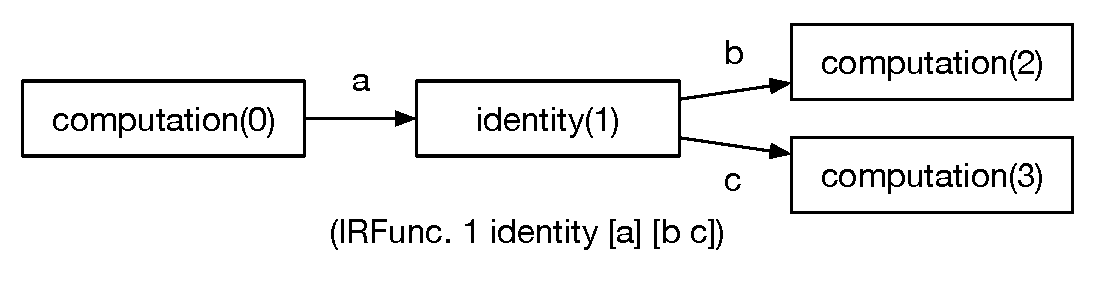
\includegraphics[width=\linewidth]{../Figures/identity-example}
    \caption{Identity use example}
    \label{fig:identity-example}
\end{figure}

\begin{figure}
    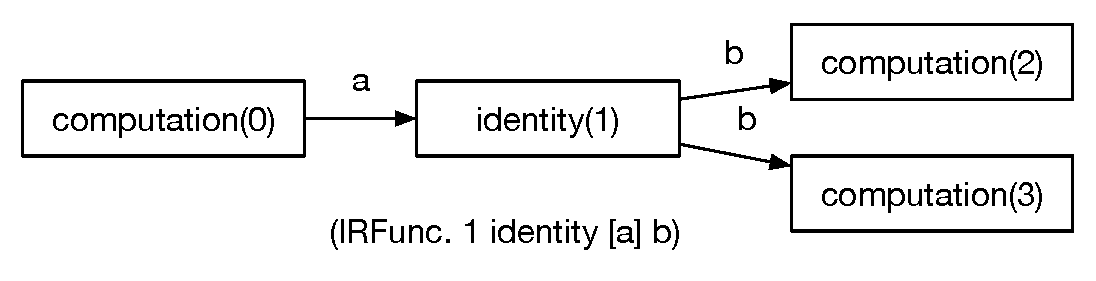
\includegraphics[width=\linewidth]{../Figures/redundant-identity-example}
    \caption{Redundant identity example}
    \label{fig:redundant-identity-example}
\end{figure}

\begin{figure}
    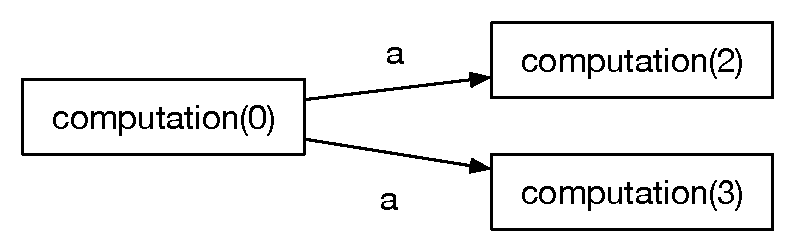
\includegraphics[width=\linewidth]{../Figures/redundant-identity-example-rewritten}
    \caption{Optimised flow}
    \label{fig:redundant-identity-example-rewritten}
\end{figure}

A second \texttt{identity} optimisation is the removal of duplicate identities.
If two identities with the same input are destructured into the same output they are redundant.
Both are removed from the graph and data is destructured at the source.
Both context arcs are connected to the respective recipients.

%!TEX root = ../thesis.tex
\chapter{Side Effects}
\label{ch:side-effects}

In terms of \yauhau{}, side effects are actions which modify a remote resource that \yauhau{} is configured to access.
They are called side effects because they violate the rules of referential transparency.
Referential transparency is a property of pure functions and means that the result of the overall computation does not change when the call sites of the referentially transparent functions are replaced by their result.
In \yauhau{} we make the assumption that, even though we do not control the implementation of the fetch performed by the data source or have control over the remote source, read requests are pure actions.
This allows us to cache results and remove duplicate requests.
In practice the remote resource may of course change as the program runs which is why we allow the programmer to choose an appropriate caching strategy with the desired tradeoff between performance and out-of-date errors.

\section{Current implementation}

This behaviour is similar to the behaviour of Haxl, which also caches fetch results and removes duplicate requests.
We however wanted to go one step further and provide the user with the ability to perform transformative actions on the remote resource during execution.
Effectful actions are of course already supported by Ohua, however as mentioned before it breaks the assumptions made by \yauhau{}.
Therefore the programmer would either have to accept the possibility of errors or relinquish the use of a cache, which has profound impacts on performance.

We solve this issue in \yauhau{} by specifically implementing write requests.
These special \texttt{write} operators are not only able to access the network in a user defined way, but it also informs the cache of the performed request.
When the user defines a cache he can also provide a function for how to manipulate the cache as a result of this request.
Two simple predefined actions are available by default \texttt{dropOne} and \texttt{dropAll}.
The former drops a request from the cache matching the current one and the latter clears the entire cache.

\begin{figure}[h]
\begin{minted}{Java}
/* Caches should implement both interfaces */
interface Dropable<A> {
  Dropable<A> dropOne(A a);

  Dropable<A> dropAll();
}

interface Cache {
  BiFunction<Dropable<Request>, Request, Dropable<Request>>
  getRemoveAction();
  Object get(Request r);
  Object set(Request r, Object resp);
  void handleStore(Request r);
  int cacheSize();
}
\end{minted}
\caption{The cache interface}
\label{fig:the-cache-interface}
\end{figure}

\section{Enforcing intra algorithm order}

The mentioned cache handling allows programmers to obtain correct read-write semantics.
However there are still issues due to ordering.
In Ohua order of execution is only guaranteed for operators with explicit data dependencies.
In the example in Figure~\ref{fig:independent-actions-code} for instance it is entirely indeterministic whether the read or write is going to be executed first.
This problem can be avoided by using an operator called \texttt{seq}.
\texttt{seq} enforces its first argument to be fully evaluated before allowing its second argument to be evaluated.
The inspiration for this operator comes from Haskell, which has a function called \texttt{seq}, however the semantics are subtly different.
Whereas Haskell's \texttt{seq} only guarantees that then it returns its second arguments both arguments have been evaluated to WHNF, Ohua's \texttt{seq} guarantees that \emph{before} the latter argument is being evaluated the first has been \emph{fully} evaluated.
In the example Figure~\ref{fig:enforcing-order-with-seq} we enforce the write to happen first using seq.

\begin{figure}[h]
\begingroup
\definecolor{green(html/cssgreen)}{rgb}{0.0, 0.5, 0.0}
\catcode`\@=\active
\def@#1@{\textcolor{green(html/cssgreen)}{#1}}
\begin{minted}[escapeinside=||]{Clojure}
(|@defalgo@| reqs [req]
  (let [_ (write req)
        r (read req)]
    r))
\end{minted}
\endgroup
\caption{Example for if independent actions}
\label{fig:independent-actions-code}
\end{figure}

\begin{figure}[h]
  \begin{subfigure}{\textwidth}
\begingroup
\definecolor{green(html/cssgreen)}{rgb}{0.0, 0.5, 0.0}
\catcode`\@=\active
\def@#1@{\textcolor{green(html/cssgreen)}{#1}}
\begin{minted}[escapeinside=||]{Clojure}
(|@defalgo@| reqs [req]
  (let [w (write req)
        r (seq w (read req))]
    r))
\end{minted}
\endgroup
\caption{Enforcing order using seq}
\label{fig:enforcing-order-with-seq}
\end{subfigure}
\begin{subfigure}{\textwidth}
\begingroup
\definecolor{green(html/cssgreen)}{rgb}{0.0, 0.5, 0.0}
\catcode`\@=\active
\def@#1@{\textcolor{green(html/cssgreen)}{#1}}
\begin{minted}[escapeinside=||]{Clojure}
(|@defalgo@| req [req]
  (read (write req)))
\end{minted}
\endgroup
\caption{Enforcing order with data dependencies}
\label{fig:enforcing-order-with-dd}
\end{subfigure}
\end{figure}

We could also achieve the same semantics by introducing data dependencies between the two function calls as seen in Figure~\ref{fig:enforcing-order-with-dd}.
These are typical semantics as would be expected of a program written in a non sequential language such as Ohua or Haskell due to laziness.
However one problem remains.

\section{Enforcing order inter algorithm}

What if we have a similar situation as above, but the read and write requests are in two algorithms?
An example of this may be seen in Figure~\ref{fig:reads-and-writes-in-algos}.
Here we have basically the same situation as above, but this time the programmer tried to introduce the data dependency by making one algorithm depend on the result of the other.
Semantics of most languages, such as, again, Haskell for instance, this should work.
However in Ohua all algorithms are directly spliced into the main program except for two boundary operators called \texttt{algo-in} and \texttt{algo-out}.
The boundary operators however only track in and output to the alorithm.
An independent fetch like the one we have here in \texttt{does-read} has no data dependency to the algorithm boundary.
As the result of our write request is only connected to the algorithm boundary, via a parameter, there is no data dependency between the read and the write request after splicing.

If as a result the order of the \texttt{read} and \texttt{write} request was nondeterministic it would be counterintuitive to the programmer.
He would expect regular program semantics to hold in this case, which they do not do.
There is of course still the \texttt{seq} operator, which we could use to enforce ordering and that would work even across algorithms, but require additional work from the programmer.
Therefore we would like to automate the addition of \texttt{seq} operators in the program where there are independent reads or writes that may cause unexpected indeterminism.

\begin{figure}
\begingroup
\definecolor{green(html/cssgreen)}{rgb}{0.0, 0.5, 0.0}
\catcode`\@=\active
\def@#1@{\textcolor{green(html/cssgreen)}{#1}}
\begin{minted}[escapeinside=||]{Clojure}
(|@defalgo@| does-read [req some-data]
  (let [res (read some-constant)]
    (computation res req some-data)))

(|@defalgo@| does-write [req]
  (write req))

(|@defalgo@| reqs [req]
  (does-read req (does-write req)))
\end{minted}
\endgroup
\caption{Reads and writes in algorithms}
\label{fig:reads-and-writes-in-algos}
\end{figure}

\section{Rewrite}

Fundamentally we only need to \texttt{seq} algorithms together when we have one of the typical read after write, write after write or read before write conflicts and the latter operator is data independent from the former.
Therefore we must first identify the dependency relationships between the algorithms.

We build a directed graph of data dependencies between algorithms by first finding all distinct algorithm context frames which have been assigned in the dataflow graph of our program.
These context frames become the nodes of our dependency graph, which is a directed graph where edges represent data flowing from the source algorithm to the target algorithm.
Edges are calculated by first finding algo exit nodes, called \texttt{algo-out}.
From an \texttt{algo-out} node we traverse the data dependencies of the program graph downwards until we either

\begin{itemize}
  \item encounter an \texttt{algo-in} node, in which case we insert an edge from the algorithm belonging to the \texttt{algo-out} node we started from to the algorithm belonging to the \texttt{algo-in} node we just encountered, into the dependency graph.
    We do not explore this path further since following dependencies are guaranteed to be covered by transitive relationships.
  \item encounter an \texttt{algo-out} node, in which case we are nested in another algorithm and we stop exploring this path since subsequent dependencies are covered by the enclosing algorithm.
\end{itemize}

Thus we obtain a version of a dataflow graph which only shows data dependencies between algorithms.

Following that we assign labels to each algorithm indicating whether the algorithm in question performs reads and, or writes.
This is done by compiling sets of algos with reads and writes.
I filter the IR function list for \texttt{fetch} and \texttt{write} nodes.
Map each node to its associated algo contexts, concatenate these and finally remove duplicate entries.
Now we have a set of read and write performing algos respectively.
Each algorithm in the graph is then labeled with \texttt{:does-read} and \texttt{:does-write} depending on which set it is member of.

Finally for each algorithm which writes the algorithm gets \texttt{seq}'ed to its algorithm boundary.
All subsequent reading algorithms, which are not dependent on another write get \texttt{seq}'ed to the writing algorithms return value.

%!TEX root = ../thesis.tex
\chapter{Conditionals}
\label{ch:Conditionals}


As of late a fair amount of work has gone into understanding exactly how the different frameworks handle conditionals.
This is of particular interest because the code generator generates conditionals in a certain form and we would like to understand how that is translated in each framework.

\section{Semantics of generated code}

Currently the code generator produces conditional code as seen in Figure~\ref{fig:generated-conditional-yauhau} for Yauhau and Figure~\ref{fig:generated-conditional-haxl} for Haxl.
From the Haxl example it is particularly obvious that values on both branches of the conditional are precomputed, that is the (monadic) operations necessary to compute both values are performed before the condition is being evaluated.
This has the consequence that any IO operation which is necessary to produce this value is performed before the condition for the \texttt{if} is evaluated and therefore might render the IO actions redundant if the value is not selected.
Of course the value might also be used in other, subsequent calculations, in which case precomputing is sensible.
In fact that is the reason why the graph serialisation in the code generator uses this particular style of code.
It does not inquire how many other nodes depend on the result of this calculation and hence obtains no evidence of whether it is safe move the computation onto the if branch itself.
As a recapture, we know now that the code generator produces conditional code for Haxl, were all branches are precomputed.
Following from the semantics of the Haxl framework all IO actions have already been performed on both values when the condition is evaluated and a branch is selected.

\begin{figure}
\begin{minted}{Clojure}
(let [val1 (computation ...)
      val2 (computation ...)]
  (if condition val1 val2))
\end{minted}
\caption{Generated conditional code for Yauhau}
\label{fig:generated-conditional-yauhau}
\begin{minted}{Haskell}
do
  (val1, val2) <- (,) <$> computation ... <*> computation ...
  return $ if condition then val1 else val2
\end{minted}
\caption{Generated conditional code for Haxl}
\label{fig:generated-conditional-haxl}
\end{figure}

\begin{figure}
  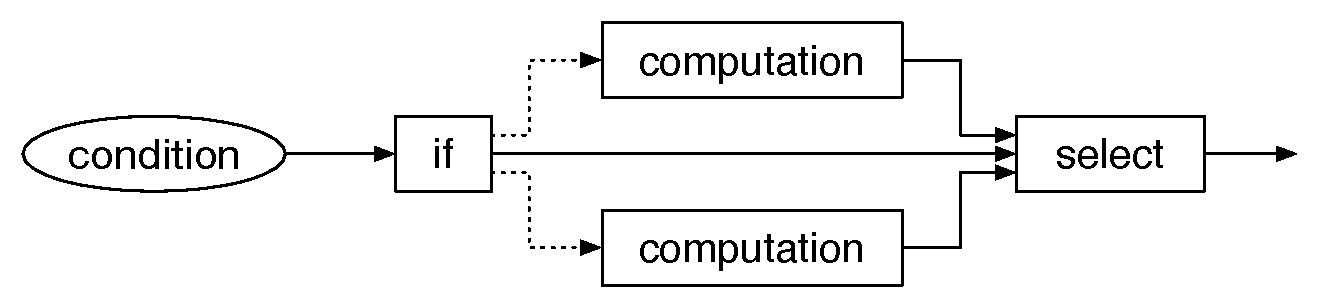
\includegraphics[width=\textwidth]{../Figures/if-hypothesised}
  \caption{Conditionals as hypothesised}
  \label{fig:if-graph-hypothesised}
  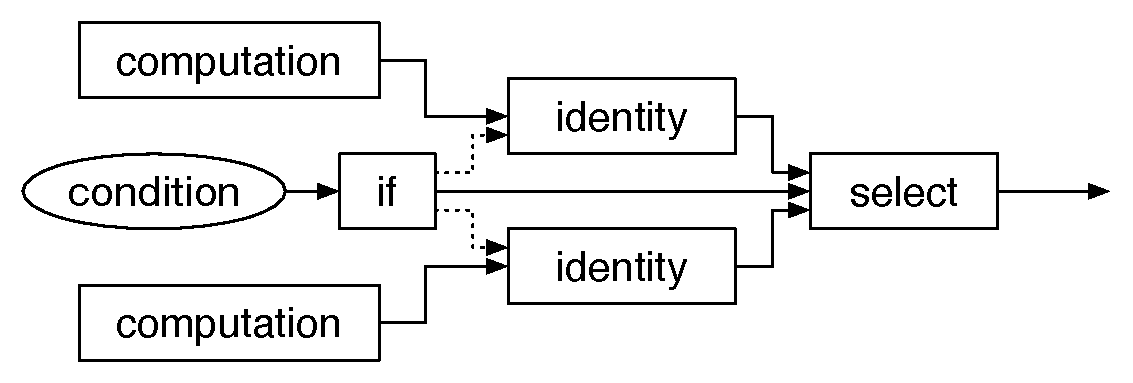
\includegraphics[width=\textwidth]{../Figures/if-in-reality}
  \caption{Conditionals actual}
  \label{fig:if-graph-actual}
\end{figure}

For a long time we suspected \yauhau{} and Ohua would handle this situation differently and \textbf{not} precompute the values, delay IO actions and only perform necessary calculations after evaluating the condition.
The reason we would come to this Hypothesis is because we thought operating on a dataflow graph would provide us with the necessary information and semantics by default.
However recently I discovered that, due to the way that Ohua translates code into graph, we do not in fact differ from Haxl in semantics.
As an example we will take the program from Figure~\ref{fig:generated-conditional-yauhau}.
We previously expected it to translate the program into a graph like the one in Figure~\ref{fig:if-graph-hypothesised}.
Here both computations are dependent on the \texttt{if} via a \textit{context arc} (dotted arrow) and therefore would be computed \textit{after} the condition had been evaluated.
The way in which Ohua would actually translate the program however would be to insert an operator called \texttt{value} on each of the if branches, which essentially wraps the bindings \texttt{val1} and \texttt{val2} respectively.
Additionally two \textit{context arcs} would be connected from the \texttt{if} to those \texttt{value} operators.
A visual representation of this can be seen in Figure~\ref{fig:if-graph-actual}.
At runtime, depending of the value of the condition, one of those \textit{context arcs} would be activated selecting the branch it is connected to, in this case the respective \texttt{value} operator.
In layman's terms the \texttt{if} selects one binding out of two at runtime, not one computation, as previously hypothesised.

We had also planned to show experiments later comparing the different semantics of \yauhau{} and Haxl when it comes to conditionals and discuss advantages and disadvantages of both.
Resulting from the recent unveilings however this has become redundant.
As much of a failure this may seem there is valuable information to be found in this.
Since we hypothesised these two different semantics we put additional thought into advantages and disadvantages of precomputing possibly unused values.


\section{Evaluation of precomputed conditional branches}

Let us assume that, in the system using Haxl or \yauhau{} computations are pure and the only stateful actions are the IO actions performed using the framework.
This view is of course not entirely consistent with reality, since nothing prevents you from doing effectful things in \yauhau{}, however in the domain where this system may be used it is a reasonable assumption to make for the purposes of the following deliberations.
Furthermore we may assume our fetches/reads to be \textit{pure} in so far as that they do not mutate the resource they request data from and serving a cached copy of a request is equivalent to actually performing the request.
How \yauhau{} deals with cases in which these assumptions do not hold is explained in detail in other chapters.

If we assume the mentioned, lets call it \textit{near purity}, we can start to consider code reordering as an optimisation.
In particular reordering code around conditional statements is a possible code optimisation.
It turns out that, when performing batching transformations, like we do, moving requests out of, or into conditional branches has more intricate and interesting effects than it would in a regular program.

Consider a simple example (Figure~\ref{fig:requests-on-branches}) where we have a regular conditional statement and depending on the result of the computation one request.
Consider how this program would be batched.
The requests on the branches depend on the the evaluation of the condition and the condition depends on the data from \texttt{request0}, see also Figure~\ref{fig:requests-on-branches-graph}.
Fetch rounds are indicated by the blue, dashed rectangle.
As a result we would end up with two fetch rounds.
One for the request before the conditional and one for either the request from the true branch or the false branch.

\begin{figure}
\begin{minted}{Clojure}
(let [data1 (get-data request0 source1)]
  (if (computation data1)
    (get-data request1 source1)
    (get-data request2 source2)))
\end{minted}
\caption{Requests on branches}
\label{fig:requests-on-branches}
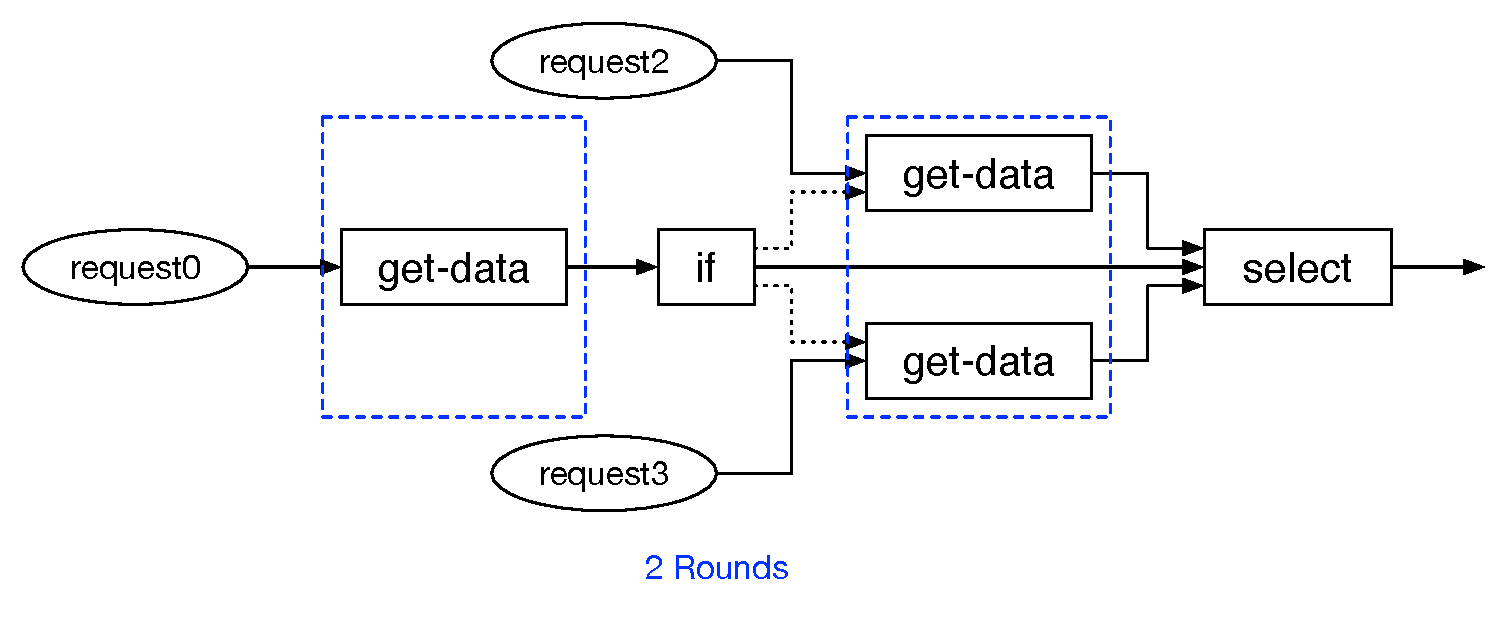
\includegraphics[width=\textwidth]{../Figures/requests-on-branches-graph}
\caption{Request on branches as graph}
\label{fig:requests-on-branches-graph}
\end{figure}

In \yauhau{} we generally operate under the assumption that IO actions are expensive.
The goal of our system is to do as few actual IO actions as possible.
In this case we see that we are performing two actions where we might only have to perform one action.
If we can, as previously mentioned, consider the fetches and computations as pure, we can rewrite the program to perform the conditional fetches \textbf{before} evaluating the condition (See Figure~\ref{fig:requests-precomputed}), which allows it to be batched with the first request, since the two fetches now do not depend on the condition anymore, See Figure~\ref{fig:requests-precomputed-graph}.
The round again indicated by the blue, dashed rectangle.
For pure computations this will be semantically identical even though it performs redundant computation.

\begin{figure}
\begin{minted}{Clojure}
(let [data1 (get-data request0 source1)
      data2 (get-data request1 source1)
      data3 (get-data request2 source2)]
  (if (computation data1)
    data2
    data3))
\end{minted}
\caption{Requests precomputed}
\label{fig:requests-precomputed}
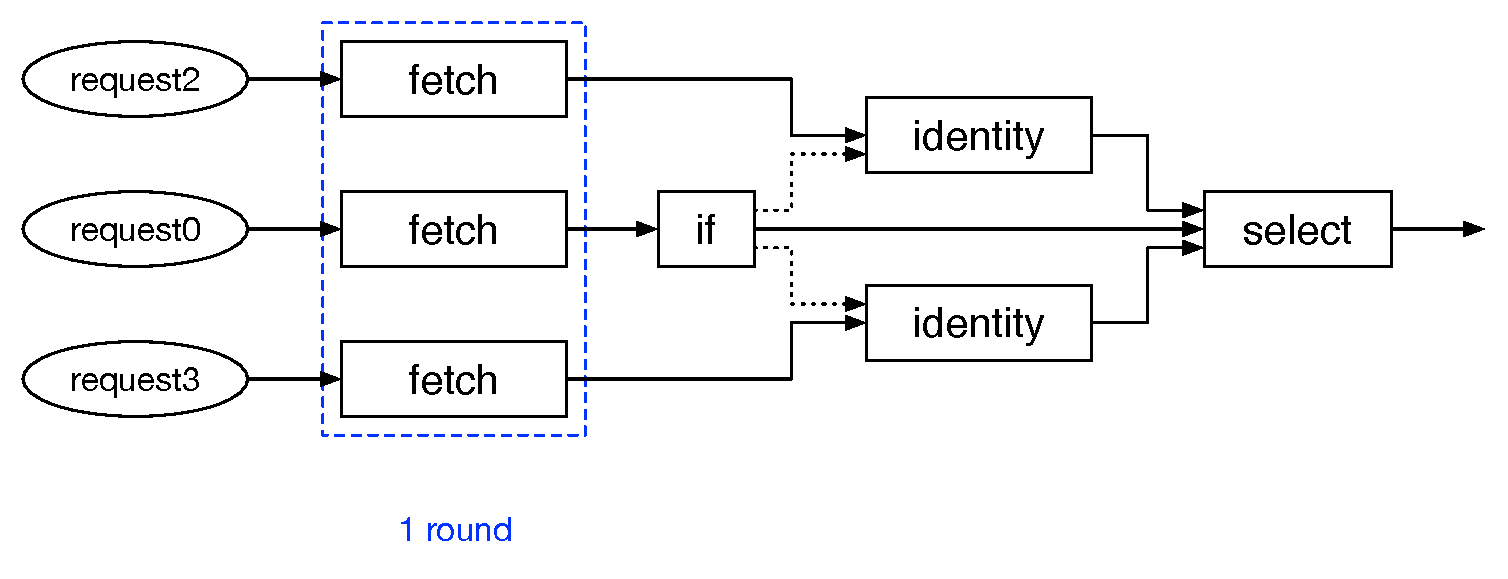
\includegraphics[width=\textwidth]{../Figures/requests-precomputed-graph}
\caption{Precomputed requests as graph}
\label{fig:requests-precomputed-graph}
\end{figure}

For many programs in our domain the latter version will be more efficient.
In particular if the fetch round before already includes a request to \texttt{source2} as well, then after our rewrite we get all the data from the entire second round for free.

However this is not always the case.
If the earlier round does not contain a request to \texttt{source2} already we would be performing an additional IO action.
It will run in parallel to the request to \texttt{source1} and thus seldom create additional latency, however if \texttt{source2} is significantly slower than \texttt{source1} our change could introduce a lot of additional latency into the program.

\begin{itemize}
  \item Rewrite from before branch to branch
  \item or rewrite from branch to precompute
  \item both require functions to be pure
  \item \texttt{@Pure} annotation?
\end{itemize}

%!TEX root = ../thesis.tex
\chapter{Extending the code generator}

\label{ch:extending-code-generator}

\section{Maps}

Adding meaningful mapping operations to is difficult.
Meaningful mappings should be done over a large collection.
However at the present the code we generate does not produce large mappable structures.
It deals mostly with small numeric values to avoid having to deal with the type system too much when generating code.

\subsection{Current status}

The code generated by our generator is determined by two things

\begin{enumerate}
    \item \textbf{The label of the node} determines the type of function call the node will be compile to.
          It holds potential extra information necessary for this type of function.
    \item \textbf{The successors} become the arguments to the function. Hence they control how many and which arguments a function receives.
\end{enumerate}

Return values of functions are never large mappable structures, as mentioned above.
Therefore we have to build mappable structures specially for map operations.
However the only data available to us to do that with are the successors to our node.
Therefore we could only build mappable structures as large as the number of successors to our node.
In order to attain reasonably sized programs however the number of successors a node can have is limited to a maximum of 6.
Lastly Ohua is currently unable to handle mapping over empty collections and also sometimes issues arise when mapping over collections of only one element, therefore we have to ensure that the generator tool does not generate maps over empty collections and for safety reasons also no collections with only one element.

When the appropriate command line parameters are given the generator randomly assigns the \texttt{Map} computation type to nodes.
I have now tweaked the serialiser, which turns the graphs into actual source code to wrap the successors of the node into collections and generate a new independent function with which to map over the collection.
Furthermore the generator has been tweaked to fix the arity for independent functions which are used for mapping to 2.
This restriction is necessary since neither Haskell nor Ohua, our two main targets for code generation support multiple arity mapping.
See produced code in Figure~\ref{fig:generated-map-code}.

\begin{figure}
\begin{minted}{Clojure}
(defalgo ifnlocal3 [param1]
    ...)
(defn main []
  (ohua
    (length (smap ifnlocal3 (vector local4 local5 local6)))))
\end{minted}
\begin{minted}{Haskell}
ifnlocal3 param1 = ...
main = do
    a <- mapM ifnlocal3 [local4, local5, local6]
    return (length a)
\end{minted}
\caption{Example for generated mapping code in Ohua and Haskell}
\label{fig:generated-map-code}
\end{figure}

\section{Pattern based generation}

\begin{itemize}
  \item We would like to generate different code for different experiments, adhering to particular patterns
  \item Future work, but should be quickly described here.
\end{itemize}

%!TEX root = ../thesis.tex
\chapter{Experiments}

\label{ch:Experiments}

In this chapter I will show some experimental evidence of the effectiveness of the system which we have implemented.
Experiments are usually run against the competing systems Haxl\cite{Haxl:library:link}.
As mentioned in previous Chapters the code used for testing all systems in equal conditions is generated with our random code generator\cite{Goens-rand-code-graph}.
Additional boilerplate implementations for test data sources etc can be found in the \yauhau{} repository\cite{Yauhau:repository:link} for the \yauhau{} experiment code and for Haxl in the haxl-test-generated-graph\footnote{https://github.com/JustusAdam/haxl-test-generated-graph} repository.

% \section{Functions}
%
% This experiment shows the effectiveness of the round-detection algorithm on modularised code by generating program graphs which contains calls to algorithms.
% Our experiment setup for this experiment operates on several graphs of constant depth (number of levels is constant).
% We gradually increase the relative amount of algorithm calling nodes in the graph.
% Additionally we run the series against multiple seeds to get an average result, hence fractional amounts of rounds.
%
% \begin{figure}[h]
%     \includegraphics[width=\linewidth]{../Figures/func-experiment.eps}
%     \caption{Number of rounds performed with functions enabled}
%     \label{fig:experiment-functions}
% \end{figure}
%
% As is visible in the graph in Figure~\ref{fig:experiment-functions} our algorithm performs better than Haxl.
% This is due to restrictions of using a runtime detection.
% In Haxl the fetches inside a called function can only be inspected once all function parameters were provided and the term was bound to the monad.
% Fetches which were independent from the function arguments therefore can still only be executed once the function received all input parameters
% Since our algorithm operates on a dataflow graph and splices algorithms we can detect fetches which are independent from algorithm arguments and perform them before the algorithm would even be called.

\section{Smap}

This experiment show the quality of transformation for program graphs containing operations which map over a collection.
Our experiment setup for this experiment operates on several graphs of constant depth (number of levels is constant).
We gradually increase the relative amount of mapping operations in the graph.
Additionally we run the series against multiple seeds to get an average result.

In order to show that we in fact achieve the same performance with maps as Haxl does we run this experiment in two configurations.
For both configurations we operate on the same code graphs.
After the graphs have been generated we randomly select a number of nodes, with probabilities as listed on the x-axis in the plots.
We then change the type, and therefore the behaviour of those nodes, in two ways.

\begin{enumerate}
  \item The designated nodes become function invocations. Figure~\ref{fig:smap-experiment-primer}
        This is equivalent to attaching a small random subgraph to the node which is run once.
  \item The designated nodes become a an invocation of a mapping operation, \texttt{mapM} in Haxl and \texttt{smap} in \yauhau{}, over a function. Figure~\ref{fig:smap-experiment}
\end{enumerate}

\begin{figure}[h]
  \begin{subfigure}{\textwidth}
      \includegraphics[width=\linewidth]{../Figures/smap-primer-experiment.eps}
      \caption{Rounds created with functions}
      \label{fig:smap-experiment-primer}
  \end{subfigure}

  \begin{subfigure}{\textwidth}
      \includegraphics[width=\linewidth]{../Figures/smap-experiment.eps}
      \caption{Number of rounds performed with maps enabled}
      \label{fig:smap-experiment}
  \end{subfigure}
\end{figure}

For each node the invoked function and the mapped function are identical in both configurations, only the number of invocations changes.
In the first configuration, Figure~\ref{fig:smap-experiment-primer}, we can then see the flat performance advantage of \yauhau{} over Haxl independent from any \texttt{smap} or \texttt{mapM}.
We use this data to correct the data from the second experiment by this advantage to only get performance with respect to mapping operations.

In the second experiment, Figure~\ref{fig:smap-experiment}, we run the same graph as in the fist experiment, but here the nodes which used to be function invocations are now mappings.
The raw result data is then corrected by the difference from the previous experiment.
For each percentage of function/mapping nodes the difference in rounds created in the first experiment (Figure~\ref{fig:smap-experiment-primer}) is subtracted from the amount of rounds created for Haxl in the second experiment (Figure~\ref{fig:smap-experiment}).
This accounts for the flat benefit which \yauhau{} gains from the code style independence.
As is visible in the plot in Figure~\ref{fig:smap-experiment} the performance of \yauhau{} and Haxl with respect to mapping operations is identical to that of Haxl.

\section{Conditionals}

Understanding exactly how the different frameworks handle conditionals is of particular interest because it may holds potential opportunity for optimisation.

\subsection{Semantics of generated code}

Currently the code generator produces conditional code as seen in Figure~\ref{fig:generated-conditional-yauhau} for Yauhau and Figure~\ref{fig:generated-conditional-haxl} for Haxl.
From the Haxl example it is particularly obvious that values on both branches of the conditional are precomputed, that is the (monadic) operations necessary to compute both values are performed before the condition is being evaluated.
This has the consequence that any I/O operation which is necessary to produce this value is performed before the condition for the \texttt{if} is evaluated and therefore might render the I/O actions redundant if the value is not selected.
Of course the value might also be used in other, subsequent calculations, in which case precomputing is sensible.
In fact that is the reason why the graph serialisation in the code generator uses this particular style of code.
It does not inquire how many other nodes depend on the result of this calculation and hence obtains no knowledge of whether it is safe to move the computation onto the if branch itself.

\begin{figure}[h]
\begin{subfigure}{\textwidth}
\begin{minted}{Haskell}
do
  (val1, val2) <- (,) <$> computation ... <*> computation ...
  return $ if condition then val1 else val2
\end{minted}
\caption{Generated conditional code for Haxl}
\label{fig:generated-conditional-haxl}
\end{subfigure}

\end{figure}


\begin{figure}
  \begin{subfigure}[b]{.5\textwidth}
\begin{minted}{Clojure}
(let [val1 (computation ...)
      val2 (computation ...)]
  (if condition val1 val2))
\end{minted}
  \caption{Generated conditional code for Yauhau}
  \label{fig:generated-conditional-yauhau}
  \end{subfigure}
  \begin{subfigure}[b]{0.5\textwidth}
    \includegr{if-in-reality}
    \caption{Graph representation}
    \label{fig:if-graph-actual}
  \end{subfigure}
\end{figure}

\begin{figure}
  \begin{subfigure}{\textwidth}
\begin{minted}{Clojure}
(let [data1 (get-data request0 source1)]
  (if (computation data1)
    (get-data request1 source1)
    (get-data request2 source2)))
\end{minted}
    \caption{Requests on branches}
    \label{fig:requests-on-branches}
  \end{subfigure}
  \begin{subfigure}{0.5\textwidth}
    \includegr{if-hypothesised}
    \caption{Conditionals as hypothesised}
    \label{fig:if-graph-hypothesised}
  \end{subfigure}
\end{figure}

The code generated for \yauhau{}, see Figure~\ref{fig:generated-conditional-yauhau} gets translated into a dataflow graph with very similar semantics to those of Haxl.
A visual representation of this can be seen in Figure~\ref{fig:if-graph-actual}.

As an example we will take the program from Figure~\ref{fig:generated-conditional-yauhau}.
However a simple change to the \yauhau{} code, see Figure~\ref{fig:requests-on-branches} can produce a graph with a different structure, see Figure~\ref{fig:if-graph-hypothesised}.

In the second version both computations are dependent on the \texttt{if} via a \textit{context arc} (dotted arrow) and therefore would be computed \textit{after} the condition had been evaluated.
In the first version the computations do not depend on the \texttt{if} and there is no context arc, instead the context arc goes to the \texttt{identity} operator which itself does nothing but return its value.
What this does as a result is select one of the two computed values, depending on the condition.
In summary: In version one the \texttt{if} selects one one \emph{computation} out of two, and in version two one \emph{binding} out of two.


\subsection{Evaluation of precomputed conditional branches}

\label{sec:precomp-eval}

Let us assume that, in the system using Haxl or \yauhau{} computations are pure and the only stateful actions are the I/O actions performed using the framework.
This view is of course not entirely consistent with reality, since nothing prevents you from doing effectful things in \yauhau{}, however in the domain where this system may be used it is a reasonable assumption to make for the purposes of the following deliberations.
Furthermore we may assume our fetches/reads to be \textit{pure} in so far as that they do not mutate the resource they request data from and serving a cached copy of a request is equivalent to actually performing the request.
How \yauhau{} deals with cases in which these assumptions do not hold is explained in detail in Chapter~\ref{ch:side-effects}.

If we assume the mentioned, lets call it \textit{near purity}, we can start to consider code reordering as an optimisation.
In particular reordering code around conditional statements is a possible code optimisation.
It turns out that, when performing batching transformations, like we do, moving requests out of, or into conditional branches has more intricate and interesting effects than it would in a regular program.

\subsubsection{New batching opportunities}

\begin{figure}[h]
  \begin{subfigure}{\textwidth}
      \includegraphics[width=\linewidth]{../Figures/if-experiment.eps}
      \caption{Round difference}
      \label{fig:if-experiment}
  \end{subfigure}
  \begin{subfigure}{\textwidth}
    \includegraphics[width=\textwidth]{../Figures/if-experiment-prct.eps}
    \caption{Round difference in percent}
    \label{fig:if-experiment-prct}
  \end{subfigure}
\end{figure}

We have made amendments to the code generator to enable us to produce both types of graph, see Section~\ref{sec:extend-conditionals}.
The experiments in Figure~\ref{fig:if-experiment} show that an absolute difference in the number of rounds which are performed in the program between when requests are precomputed and when they are not.
The figure shows an average difference in the number of performed rounds, as well as a highest and lowest value for the number of rounds saved.
The formula is always $precomputed - inline$.
Since the minimum value is never below $0$ we can conclude that the precomputed version never performs more rounds than the inlined one and on average we save three rounds of I/O when precomputing the branches.
Figure~\ref{fig:if-experiment-prct} shows the average, minimum and maximum percentage of rounds which were saved my precomputing the branches.

By precomputing branches we can decrease the number of rounds in a program on average by about 15\% and up to 25\%.
Simultaneously we can observe a significant increase in the number of performed fetches compared to the inlined version, see Figure~\ref{fig:if-experiment-fetches}.

\begin{figure}[h]
    \includegraphics[width=\linewidth]{../Figures/if-experiment-fetches.eps}
    \caption{Number of fetches performed}
    \label{fig:if-experiment-fetches}
\end{figure}

In \yauhau{} we generally operate under the assumption that I/O actions are expensive.
The goal of our system is to do as few actual I/O actions as possible.
Fewer rounds of I/O generally reduces the execution time for the program.

\subsubsection{Explanations}

Consider a simple example (Figure~\ref{fig:requests-on-branches}) where we have a regular conditional statement and depending on the result of the computation one request.
Consider how this program would be batched.
The requests on the branches depend on the the evaluation of the condition and the condition depends on the data from \texttt{request0}, see also Figure~\ref{fig:requests-on-branches-graph}.
Fetch rounds are indicated by the blue, dashed rectangle.
As a result we would end up with two fetch rounds.
One for the request before the conditional and one for either the request from the true branch or the false branch.

In this case we see that we are performing two actions where we might only have to perform one action.
If we can, as previously mentioned, consider the fetches and computations as pure, we can rewrite the program to perform the conditional fetches \textbf{before} evaluating the condition (See Figure~\ref{fig:requests-precomputed}), which allows it to be batched with the first request, since the two fetches now do not depend on the condition anymore, See Figure~\ref{fig:requests-precomputed-graph}.
The round again indicated by the blue, dashed rectangle.
In particular if the fetch round before already includes a request to \texttt{source2} as well, then after our rewrite we get all the data from the entire second round for free.
For pure computations this will be semantically identical even though it performs redundant computation.

\begin{figure}[h]

  \begin{subfigure}{\textwidth}
\begin{minted}{Clojure}
(let [data1 (get-data request0 source1)
      data2 (get-data request1 source1)
      data3 (get-data request2 source2)]
  (if (computation data1)
    data2
    data3))
\end{minted}
    \caption{Requests precomputed}
    \label{fig:requests-precomputed}
  \end{subfigure}

  \begin{subfigure}{0.7\textwidth}
    \includegr{requests-precomputed-graph}
    \caption{Precomputed requests as graph}
    \label{fig:requests-precomputed-graph}
  \end{subfigure}
  \begin{subfigure}{.7\textwidth}
    \includegr{requests-on-branches-graph}
    \caption{Request on branches as graph}
    \label{fig:requests-on-branches-graph}
  \end{subfigure}
\end{figure}

\begin{figure}[h]
    \includegr{critical-path}
    \caption{Critical path of fetches}
    \label{fig:critical-path}
\end{figure}

\subsubsection{Findings and explanation}

We can save up to 25\% of rounds and an average of about 15\% of rounds by precomputing conditional branches.
However these numbers were achieved in programs with a large number of conditional nodes.
Up to 95\% (of nodes with three children) were tagged and serialised as conditional nodes.
Considering this strong bias for conditionals the results seem pretty low.

The explanation for these low numbers seem to be that pulling fetches up into an earlier round only reduces the overall number of rounds if said fetch was part of the critical fetch path.
Like the critical path in a program we can construct a graph of data dependencies where we only include \texttt{fetch} nodes.
A visual representation of this can be seen in Figure~\ref{fig:critical-path}
The number of fetches along the longest path through this graph is the critical path with respects to fetches and marks a lower bound to the number of rounds we have to perform.
If the fetches we pulled from their branches were not part of the critical path pulling them up wont change the overall number of rounds at all, compare Figure~\ref{fig:rewrite-not-crit-path}, since there would have been a necessary later round which we cannot avoid performing and which could have incorporated the fetches from our branch.
Conversely if the fetches were part of the critical path, pulling them up reduces the length of the critical path, see Figure~\ref{fig:rewrite-crit-path}, ergo the optimal solution to minimal rounds decreases and our algorithm finds it.
Note that this is not limited to fetches on the critical fetch path of the original program but also to fetches on the new critical path resulting from a rewrite.

\begin{figure}[h]

  \begin{subfigure}[b]{.5\textwidth}
    \includegr{rewrite-not-crit-path}
    \caption{Moving fetches not on the critical path}
    \label{fig:rewrite-not-crit-path}
  \end{subfigure}

  \begin{subfigure}[b]{.5\textwidth}
    \includegr{rewrite-crit-path}
    \caption{Moving fetches on the critical path}
    \label{fig:rewrite-crit-path}
  \end{subfigure}

\end{figure}

%
% In these experiments I generate particularly narrow program graphs to create dominant critical paths, i.e. one long, interconnected path (Figure~\ref{fig:dominant-critical-path}) rather than several medium length paths (Figure~\ref{fig:non-dominant-critical-path}).

In our experiments all fetches had the same execution time, however if we consider a system with fetches of heterogeneous latency we find another potential source of increased performance.
If the fetches we pulled into earlier rounds have a particularly long latency we might observe decreased execution time, even if they were not part of the critical path, since we would be increasing the amount and length of program paths able to run concurrently with the fetch.
Simultaneously however we might significantly increase runtime if we precompute a particularly expensive fetch which in the end turns out would not have been selected by its conditional.

Overall precomputing request seems a promising area for optimisation, however it would require a smart heuristic for selecting sites which are likely to yield a performance benefit and perhaps additional information about the data sources to decide whether a certain rewrite is beneficial.
This goes beyond the scope of this thesis.


%----------------------------------------------------------------------------------------
%	THESIS CONTENT - APPENDICES
%----------------------------------------------------------------------------------------

\appendix % Cue to tell LaTeX that the following "chapters" are Appendices

% Include the appendices of the thesis as separate files from the Appendices folder
% Uncomment the lines as you write the Appendices

% Appendix A

\chapter{Appendix Title Here} % Main appendix title

\label{AppendixA} % For referencing this appendix elsewhere, use \ref{AppendixA}

Write your Appendix content here.
%\include{Appendices/AppendixB}
%\include{Appendices/AppendixC}

%----------------------------------------------------------------------------------------
%	BIBLIOGRAPHY
%----------------------------------------------------------------------------------------

\printbibliography[heading=bibintoc]

%----------------------------------------------------------------------------------------

\end{document}
